%%%%%%%%%%%%%%%%%%%%%%%%%%%%%%%%%%%%%%%%%%%%%%%%%%%%%%%%%%%%%%%%%%%%%%%%%%%%%%%
%2345678901234567890123456789012345678901234567890123456789012345678901234567890
%        1         2         3         4         5         6         7         8

\documentclass[journal]{IEEEtran}  % Comment this line out
                                                          % if you need a4paper
%\documentclass[a4paper, 10pt, conference]{ieeeconf}      % Use this line for a4
                                                          % paper

%\documentclass[conference,twocolumn]{IEEEtran}

\IEEEoverridecommandlockouts                              % This command is only
                                                          % needed if you want to
                                                          % use the \thanks command
\overrideIEEEmargins
% See the \addtolength command later in the file to balance the column lengths
% on the last page of the document
\usepackage[switch]{lineno}
%
%\onecolumn

\usepackage{graphics} % for pdf, bitmapped graphics files
\usepackage{graphicx} % for pdf, bitmapped graphics files
%\usepackage[top=1in, bottom=1in, left=1in, right=1in]{geometry}
\usepackage{subfigure}
\usepackage{epsfig} % for postscript graphics files
%mathptmx package is not useful in most cases
%\usepackage{mathptmx} % assumes new font selection scheme installed: It gives ugly \sum markers
\usepackage{amsmath} % assumes amsmath package installed
\usepackage{amscd} % CD environment
\usepackage{amssymb}  % assumes amsmath package installed
\usepackage{amsfonts}  % assumes amsmath package installed
%\usepackage{amsthm}  % assumes amsmath package installed
\usepackage[linesnumbered, vlined, ruled]{algorithm2e}
\usepackage{multirow}
\usepackage{multicol}
\usepackage{booktabs}
%\usepackage{todonotes}
\usepackage[verbose]{wrapfig}
\usepackage{placeins}
%%%\usepackage[usenames, dvipsnames]{pstricks}
%%%\usepackage{pst-grad}
%%%\usepackage{pst-plot}
\usepackage{epstopdf}
\usepackage{bm}
\usepackage{url}
\usepackage{stfloats}
\usepackage{array}
\usepackage{booktabs}
\usepackage{color} % for \textcolor command
\usepackage{setspace}
%\doublespacing

\usepackage[table]{xcolor}
%\usepackage[scaled=0.92]{helvet}
%\usepackage[square, comma, sort&compress]{natbib}

%\usepackage{tikz}
%\usetikzlibrary{decorations.pathmorphing} % noisy shapes
%\usetikzlibrary{fit}pathmorphing% fitting shapes to coordinates
%\usetikzlibrary{backgrounds} % drawing the background after the foreground
%\usetikzlibrary{shapes,arrows}
%\usetikzlibrary{snakes,automata,petri}
%\usetikzlibrary{arrows,positioning}
%\usepackage{cite} 
%\usepackage[square,sort]{natbib}

\newcommand{\argmax}{\arg\!\max}
\newcommand{\argmin}{\arg\!\min}
\newcommand{\ming}[1]{\textcolor{red}{#1}}
\newcommand{\cming}[1]{\textcolor{blue}{#1}}
%\newcommand{\argmax}{\operatornamewithlimits{argmax}}
% The following packages can be found on http:\\www.ctan.org
%\usepackage{graphics} % for pdf, bitmapped graphics files
%\usepackage{epsfig} % for postscript graphics files
%\usepackage{mathptmx} % assumes new font selection scheme installed
%\usepackage{times} % assumes new font selection scheme installed
%\usepackage{amsmath} % assumes amsmath package installed


%\title{A Resource Allocation Strategy in a Cloud Robotic Network for Smart Homes
\title{An Incremental Auction-based Resource Allocation Strategy for Cloud
  Robotic Systems 
}

%\titlerunning{Short form of title}        % if too long for running head

\author{Lujia Wang$^{1}$, Ming Liu$^{2}$, Danilo
  Tardioli$^{3}$, Matthew Tan$^{4}$,  and Max Q.-H. Meng$^{5}$ %etc.

\thanks{$^{1}$Lujia Wang is with the School of Electrical and Electronic
  Engineering, Nanyang Technological University, Singapore. 
          %    Tel.: +123-45-678910\\
          %    Fax: +123-45-678910\\
          {\tt  \small wanglj@ntu.edu.sg}}           %  \\
%             \emph{Present address:} of F. Author  %  if needed
  \thanks{$^2$  
  Ming Liu  is with
  Department of Mechanical and Biomedical Engineering,
  City University of Hong Kong, Hong Kong. 
  \tt \small \{mingliu@cityu.edu.hk\}}           %  \\
  \thanks{$^3$ Danilo Tardioli is with
   Centro Universitario de la Defensa, Zaragoza. 
  \tt \small \{dantard@unizar.es\}}           %  \\
  \thanks{$^{4}$
  Matthew Tan was an exchange student at ETH Zurich and home university was
    Imperial College London.  \tt \small \{tanfhm@gmail.com\}}           %  \\
\thanks{$^{5}$Max Q.-H is with Department of Electronic Engineering, Chinese
  University of Hong Kong, Shatin N.T., Hong Kong. 
          {\tt  \small qhmeng@ee.cuhk.edu.hk}}           %  \\
}


\begin{document}
\linenumbers 

\maketitle

\begin{abstract}
Cloud robotic networks adopt decentralized approaches to avoid the
single point of failure.
The decentralized ad-hoc networks, being infrastructure-less, are fast to set
up, low cost and widespread with a much scarcer amount of bandwidth.
However, networked robots need to upload and download data efficiently to
provide services  hence implying real-time requirements. 
Therefore, a resource allocation strategy is required to fulfill these
real-time needs, especially for the cases with limited network bandwidth.
The aim is 
%two-fold: 1) to allocate the network fairly among all nodes when unmanned; 2)
%to allocate more of the network resource to a node that the user may favor over
%the other nodes. 
to allocate the network resource according to the priority of nodes influenced
by the requirement of users. 
This paper formulates an optimization problem of resource allocation including
a non-convex cost function and time constraint. 
This paper presents an auction-based resource allocation mechanism to allocate
the network resource among nodes in a cloud robotic ad-hoc network.
In particular, a leaderless consensus procedure is adopted to share the bids
among the networked robots. 
Each robot in the system locally bids for a quantity of transmission time slots
in a distributed manner.
The effectiveness of the mechanism has been tested to validate how
environmental factors can affect the performance in various indoor
environments. 
Besides, specific configurations are described, and the corresponding
performance results are presented and discussed.
\end{abstract}

\begin{keywords}
Auction, Resource allocation, Ad-hoc networks
\end{keywords}
% \PACS{PACS code1 \and PACS code2 \and more}
% \subclass{MSC code1 \and MSC code2 \and more}


\section{Introduction}
\label{intro}
Nowadays, robotic services are more complicated and diversified with rapid
evolving of social development.
It is impossible to develop a single robot that performs all expected services
with various limitations, such as power consumption, payload, sensory and
kinematic constraints. 
Various sensors equipped on a single robot are usually expensive
and power consuming.
Fortunately, robots can be relieved from equipping various sensors benefiting
from highly developed network technology because running information can be
stored and retrieved from online data centers.
Robots and Internet-of-things systems (such as systems supported by Xively
      \texttrademark and Intorobot \texttrademark) are deployed at different
locations to provide heterogeneous services, such as elderly-attendance, remote
surveillance and home automation \cite{wang2008robust}.
%Benefiting from the highly developed network, all primary information can be 
%stored and retrieved from online data centers such as a cloud.
Although the data requirements of robotic tasks on local infrastructures are 
seemingly highly alleviated by the cloud, there are still drawbacks and
challenges to be further addressed.
Robots may not always connect to an Internet-based cloud by themselves, such as
hazardous environment, tunnel environment \cite{Rizzo18092013}, etc.
Then, the ad-hoc network is selected among robots and a server because of its 
infrastructure-less and distributed features \cite{sheng2012localisation}. 
However, its limited network bandwidth is a primary hold-back in the robotic system.
Furthermore, cooperations of a task completed by a robot team have hard 
real-time communication requirements.
We consider this limited resource allocation is thus the most fundamental
problem in cloud robotic networks.

%Auction-based mechanisms have been proposed to solve the resource allocation
%problems in several fields such as economics and wireless routing, in order to
%investigate how agents make decisions in presence of competition for resources.
%Various auction algorithms, such as sequential second price auction
%\cite{morales2014revenue}, Vickrey auction \cite{stan2010coop_arq}, double auction
%\cite{nassiri2015bidding} and combinatorial auction \cite{fuji2010comb_auc}
%have been proposed and extended in various applications.

Auction-based mechanisms were first proposed in economics, where the bidding
process commonly used in most contract-based algorithms 
\cite{duan2014contractAuction}.
Auction approaches in multi-hop networks were used for the routing. %of
%transmission routing.
%For instance, Anderegg \textit{et al.} proposed Vickrey auction-based
%cost-efficient mechanism using the information of energy emission levels
%\cite{Anderegg03adhoc-vcg}; 
For example, Zhang \textit{et al.} developed an auction mechanism to encourage
cooperative data message relaying for each hop, which optimizes the total costs
for data messages routing from sources to destinations \cite{zhang2010aim}. 
Apart from auctions for optimal paths, auctions for bandwidth in Mobile
Ad-hoc Networks (MANETs) were also presented. 
%such as a generalized Vickrey auction model was proposed in
%\cite{chen2004ipass}. 
%It showed that the auction mechanism works both as an incentive for the
%router nodes to share the resource, and a flow control method in a
%non-cooperative mobile ad hoc network.
Kao \textit{et al.} presented an auction-based bandwidth allocation with
a multi-hop flow coordination mechanism to enhance various aspects
\cite{bw2011allocation}.
% distributed auction
Zavlanos \textit{et al.} proposed a parallel auction algorithm for a
distributed auction, in which only local information is available
\cite{ZavlDistAuc2008}. 
The results reveal that they always converge to an optimal solution, which
maximizes the total benefit using a linear approximation. 
Also, auctions among a large number of agents were evaluated via
simulations. 
It is yet to be seen, however, how this algorithm performs under random
environmental influences, as well as when real-time requirements have to be
fulfilled.

Researchers in robotics have been focusing on task allocation problems, which
is a subset of the field of resource allocation problems.
The Contract Net Protocol (CNP) \cite{wang2014multi} features algorithms that
allow many nodes to negotiate and agree on ``contracts'' to complete composite
tasks with each other, based on each node's current capabilities and
workloads.  It successfully introduced a general framework for using
auction-based mechanisms in cooperative robotics.
MURDOCH \cite{soldBP2002} was the first implementation on top of the CNP
framework in robotics to introduce single-round, first-price auctions for
on-line task problems (tasks that arrive at random). 
Computational costs are very low, and network resources used are linearly
related to the number of robots. 
TraderBots \cite{TraderBotsDias2003} is probably the most representative
implementation of early auction-based techniques for multi-robot coordination. 
The active use of a market economy helps to take into account changes in the
global environment in a decentralized way. 
While the CNP can be applied to any multi-agent system, MURDOCH and
TraderBots are more specific to task allocation for mobile robots. 
However, the validation of these systems does not consider applications that
require real-time data transmission.
Choi \textit{et al.} presented two consensus-based algorithms
\cite{choi2009consensus}. 
The algorithm builds a single bundle and bids included tasks based on the
improvement provided by the bundle.
It reduced the computation by considering only one single bundle while
improving convergence times by sequential auctions for the parallel assignment
of multiple tasks. 
Zack \textit{et al.} proposed an auction-based algorithm to control the 
reconfigurable teams \cite{Butler2015taskallocation}, which 
extends the traditional methods by using the dividing and merging operations
to improve the efficiency of the overall mission.
However, the algorithms are not quick enough to satisfy the hard real-time
requirements.
%Lagoudakis \textit{et al.} suggests having multiple one-round auctions to
%allocate all tasks to robots before execution \cite{lagoudakis2004simple}. 
%The algorithm is a centric one which uses six bidding rules for a single task.
%This system has an element of centrality, limiting the purposefulness of
%decentralised systems.


Other than not addressing the real-time requirements, the above works tackle
the resource allocation problem only at the application level and not at the
protocol level.
Furthermore, most of them gauge the performance of the algorithms in
simulations. 
They assume the unlimited resource can be achieved by extending the computing
units.  In fact, the extension is nontrivial because the data process and
storage infrastructure need to upgrade totally from a small-scale cloud to a
large-scale cloud. 
Some of our previous works have extensively explored this problem using
various scenarios. A co-localization case was studied in \cite{Lujia12Robio},
        where the bandwidth and sensor data were taken as shared resources
        among multiple robots.
The sensor data retrieval was specifically dealt with in
\cite{Lujia12Mfi,Lujia2015tase} as well, which was adapted to a
multi-sensor-based recognition scenario \cite{liu12dpfusion}.
In \cite{lujia2013icia}, the authors introduced an auction-based theory
for resource allocation in a tree-structured network.
In this paper, we extend these previous sets of research.
We present the incremental auction strategy working efficiently for resource
allocation for cloud robotic systems\cite{lujia2014icra}.
The proposed resource allocation strategy attempts to address this gap in
research and tests its effectiveness in a typical indoor environment.
Major parameters used in this paper are summarized in Table
\ref{tab:para_list} for quick reference. 

%\newcolumntype{L}{>{\centering\arraybackslash}m{1.6cm}}
\begin{table}[htpb]
\small
\caption{Parameter List}
\label{tab:para_list}
\begin{center}
%\begin{tabular}{cccc}
%\begin{tabular}{cccc}
%\begin{tabular}{m{3.6cm}m{2cm}LL}
\begin{tabular}{cl}
\toprule
\centering Symbols & Descriptions \\ 
\midrule
$P_{\text{ref}}$  &  The reference percentage of transmission slots \\ 
$T$  &  The deadline of the transmission \\ 
$t_i$  &  The duration of the node $i$ last transmitted \\ 
$c(t)$  &  The total cost function \\ 
$c_i(t_i)$  &  The cost function of node $i$ \\ 
$f_i(t_i)$  &  The time cost function  \\ 
$\Delta_i(t_i)$  &  The transmission cost function  \\ 
$h_i(t_i)$  & The number of hops of of node $i$ to reach the server \\ 
$a$  & The scaler of the node's hop number    \\ 
$\mathcal{G}$  &  The dynamic network communication graph \\ 
$V$ & The set of nodes in the network \\
$E$ & The set of edges in the network \\
$\pi_+$ & The injection amount that node $i$ has to spend \\
$\pi_-$ & The suppression amount that node $i$ can save \\
$\tau$ & A amount of waiting time for exchanging in the auction \\
$x^{[i]}$ & The index of node $i$ in the auction  \\
$y^{[i]}$ & The bid of node $i$ in the auction  \\
$\mathcal{N}_i$ & The set of node $i$ neighbors \\
$\beta$ & The coefficient of the reference amount of transmission slots \\
$FPS$ & The instantaneous transmission rate of frame \\
$U(t)$ & The utility function \\
$n$ & The number of nodes in the network \\
$R_f$ & The total reference number of transmission slots \\
$S_f$ & The transmission slots taken up by the favored node \\
$P_f$ & The proportion of transmission slots taken up by the  \\
 & favored node \\
\bottomrule
\end{tabular} 
\end{center}
\end{table}

It is organized as follows: 
%Section \ref{sec:rtwmp} gives an overview of the Real Time - Wireless Multi-Hop
%Protocol (RT-WMP) \cite{Danilo07rtwmp}.
Section \ref{sec:alg} formulates the resource allocation problem and describes
the proposed auction-based resource allocation strategy with a consensus
procedure. 
Section \ref{sec:incsimulation} reveals the system utility function and
determines suitable parameters for the system cost function in simulations. 
Section \ref{sec:inc_experiment} presents the experiments conducted to test
the effectiveness of the proposed strategy and present the results. 
Finally, Section \ref{sec:conclusion} concludes this paper with insights drawn
from the research and provides an overview into future work.



%\section{Benchmarking of RT-WMP}
%\label{sec:benchmarking}
%Before testing the efficacy of the proposed strategy, we performed a
%benchmarking campaign to evaluate the behavior of the protocol in different
%conditions.
%
%The main motivation for conducting these sets of benchmarking tests was to
%determine the best possible performance under the given environmental
%conditions. These benchmarking experiments also provide the readers with an
%insight on how the protocol operates under WiFi interference.
%
%In addition, the results obtained here will be used to gauge the performance of
%the resource allocation strategy developed by the author in Section \ref{sec:alg}.
%
%The experiments were conducted in two different indoor environments:
%one in an area with minimal WiFi interference, the other in an area with
%significant WiFi interference.
%%\subsection{Motivation}
%
%\subsection{Setup of Benchmarking Experiments}
%The best possible performance exhibited by the RT-WMP is attained in a network
%consisting of a single-link between two nodes. In this case, an E-puck was
%programmed to continuously transmit compressed JPEG images to a laptop that
%acted as a server at a frame rate of 7.5 Hz.
%These images took up a bandwidth of approximately 30 - 35 KB/s and were
%generated by a Point Grey Firefly Camera
%\footnote{http://ww2.ptgrey.com/USB2/fireflymv}, which was connected directly
%to the E-puck. 
%A low frame rate was deliberately chosen to ensure that the RT-WMP was able to
%keep up with the transmission of images to the server, preventing the network
%from getting saturated such that the transmission queues overflow.
%
%The operating frequency used was 2.462 GHz (or Channel 11 in the list of WLAN
%channels for 2.4 GHz). This frequency was used because it is situated far away
%from the popular 2.412GHz frequency band (Channel 1), which was typically extremely
%saturated with other existing WiFi networks, such that less meaningful results
%would be obtained at that frequency. In addition, the 2.462 GHz band is
%considered to be one of the non-overlapping channels in both 802.11b and
%802.11g/n.
%
%
%\subsection{Environment of Locations} 
%\label{sub:env_locations}
%The benchmarking experiments were carried out along the open areas on Level A
%and Level E of a building, which have different levels of interference on
%the WiFi channels. 
%At the different levels, the E-pucks were placed in increments of 5m away from the server. (Refer
%to Fig \ref{fig:benchmark_levelA_floorplan}).
%
%\subsubsection{Level A}
%
%\begin{figure}
%\centering
%\subfigure[Floor Plan]{
%  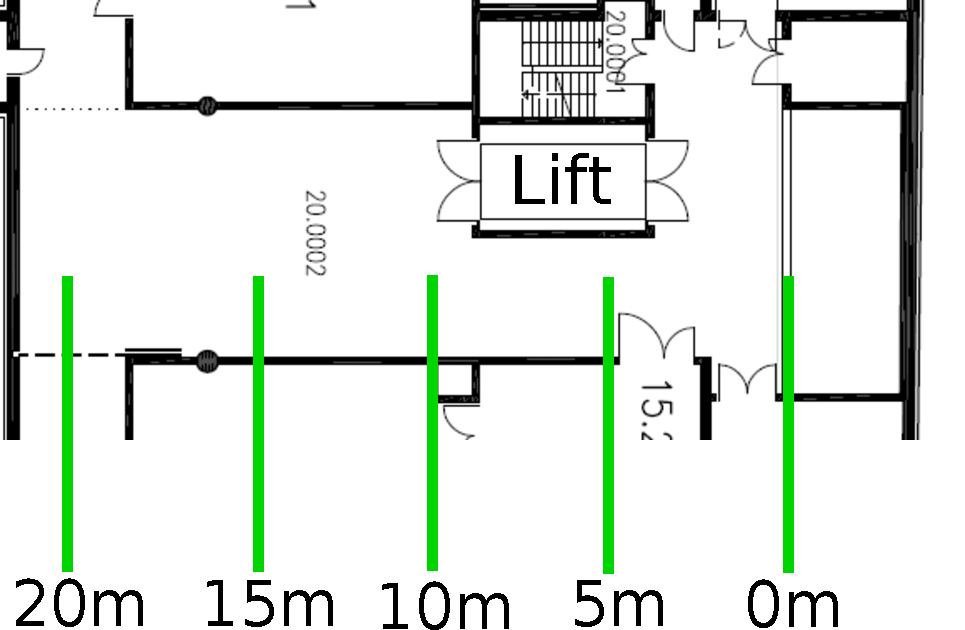
\includegraphics[angle=90,width=0.22\textwidth]{Tex_Picts/extracted_floorplan_CLA_A_benchmark.pdf}
%  \label{fig:benchmark_levelA_floorplan}
%}
%\subfigure[WiFi Trace]{
%  %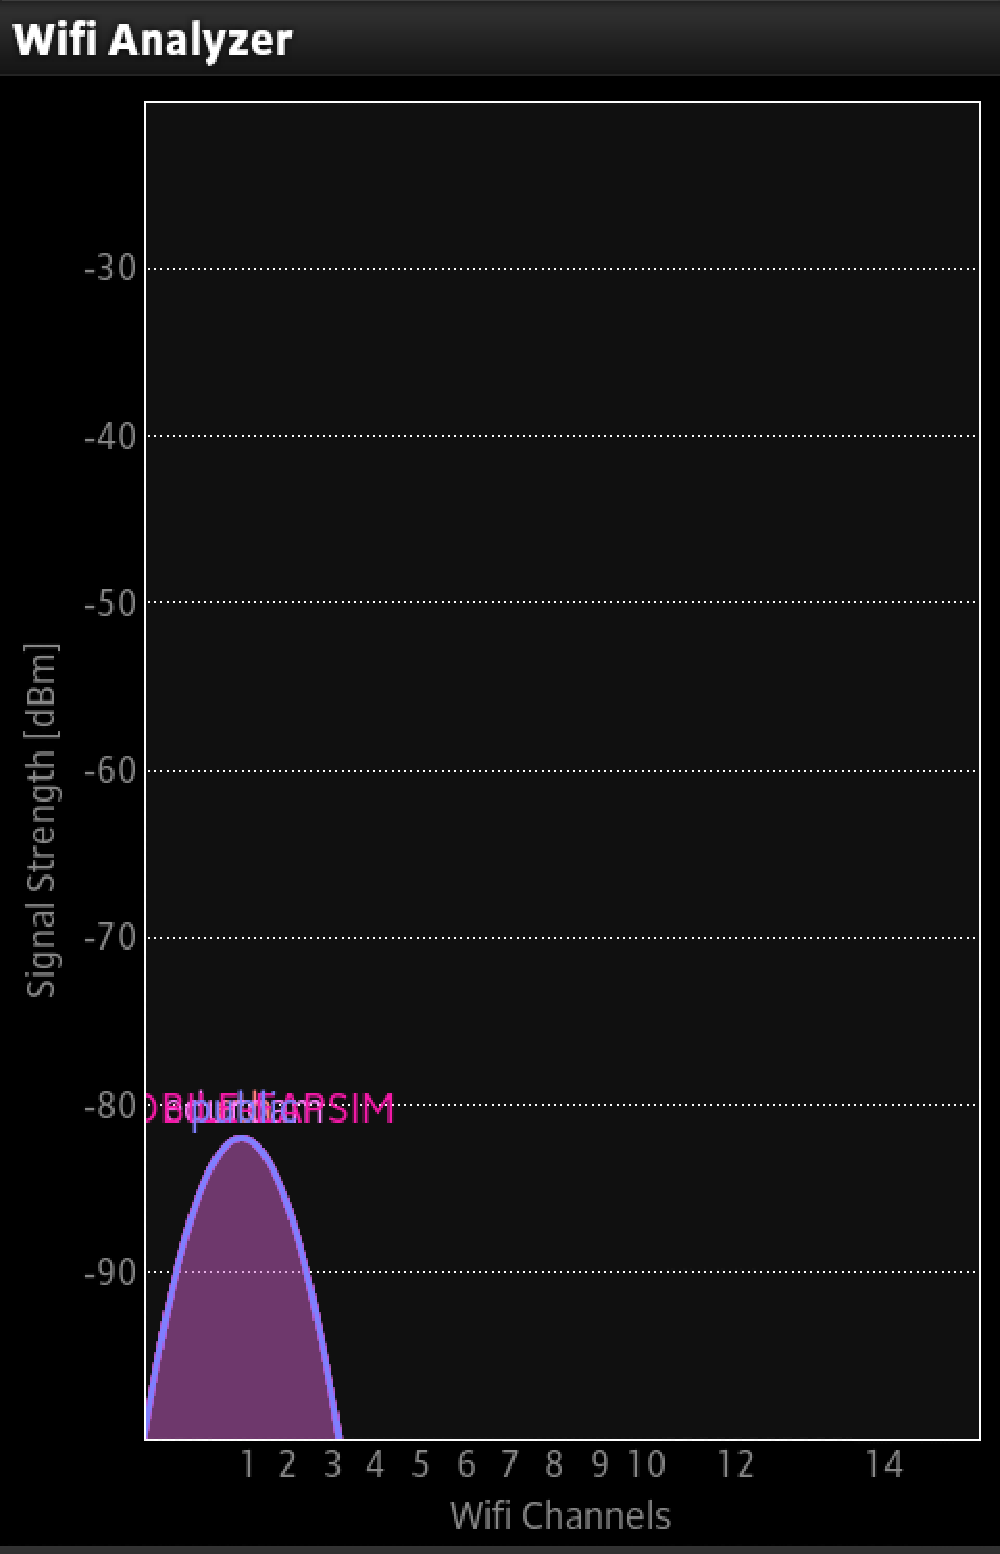
\includegraphics[width=0.22\textwidth]{Tex_Picts/levelA_edited.pdf}
%  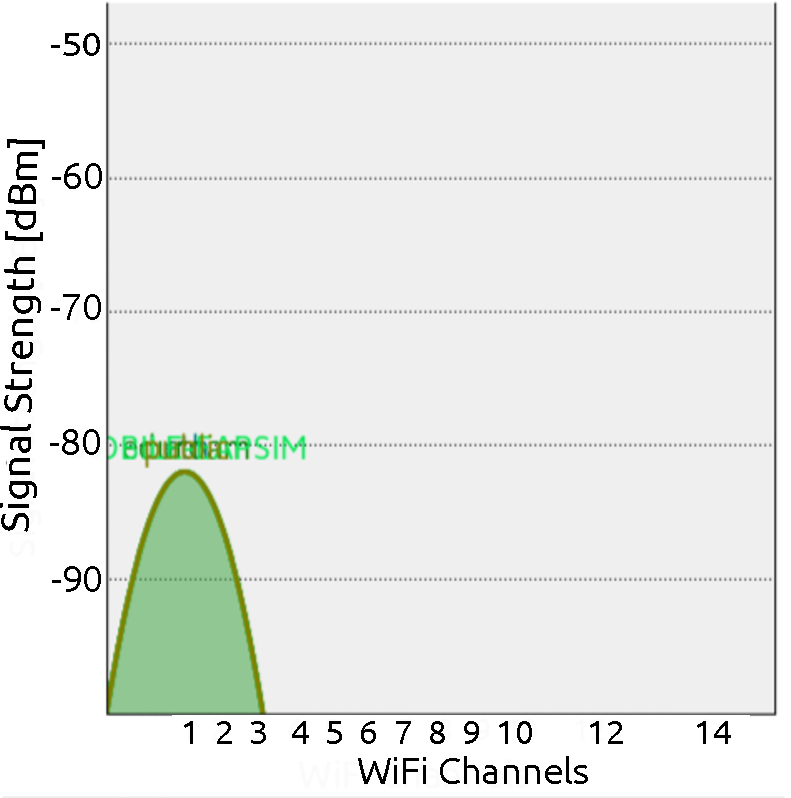
\includegraphics[width=0.46\columnwidth]{figure/levelA.pdf} 
%  \label{fig:benchmark_levelA_wifi_trace}
%}
%\caption{Benchmarking at Level A}
%\end{figure}
%
%The test area of Level A (located four levels below ground level) is a wide
%open area, mainly surrounded by concrete walls. A simple WiFi sweep was
%conducted and the trace revealed that there were no other WiFi signals present
%at the desired operating frequency (Fig. \ref{fig:benchmark_levelA_wifi_trace}).
%Thus, WiFi interference is expected to be minimal in this area.
%
%
%\subsubsection{Level E}
%
%\begin{figure}
%\centering
%\subfigure[Floor Plan]{
%  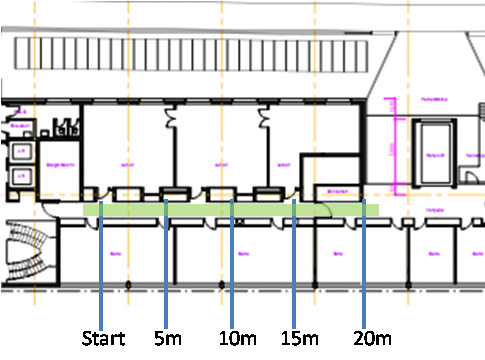
\includegraphics[angle=90,width=0.22\textwidth]{Tex_Picts/floorplan_LevelE_benchmark.pdf}
%  \label{fig:benchmark_levelE_floorplan}
%}
%\subfigure[WiFi Trace]{
%  %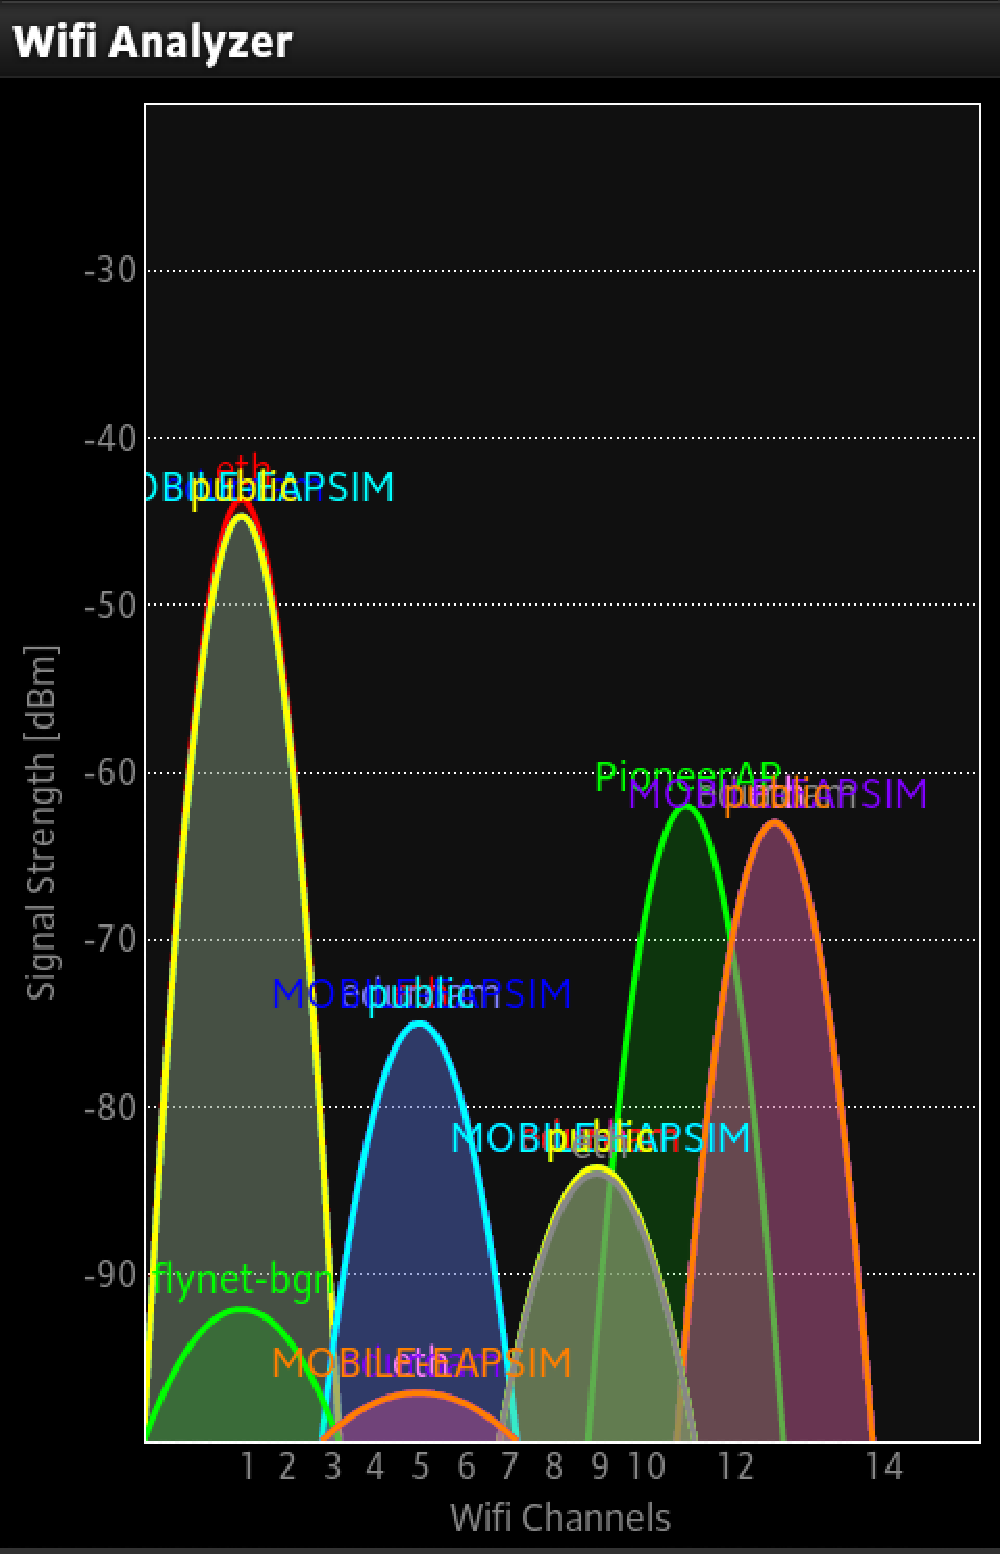
\includegraphics[width=0.22\textwidth]{Tex_Picts/levelE_edited.pdf}
%  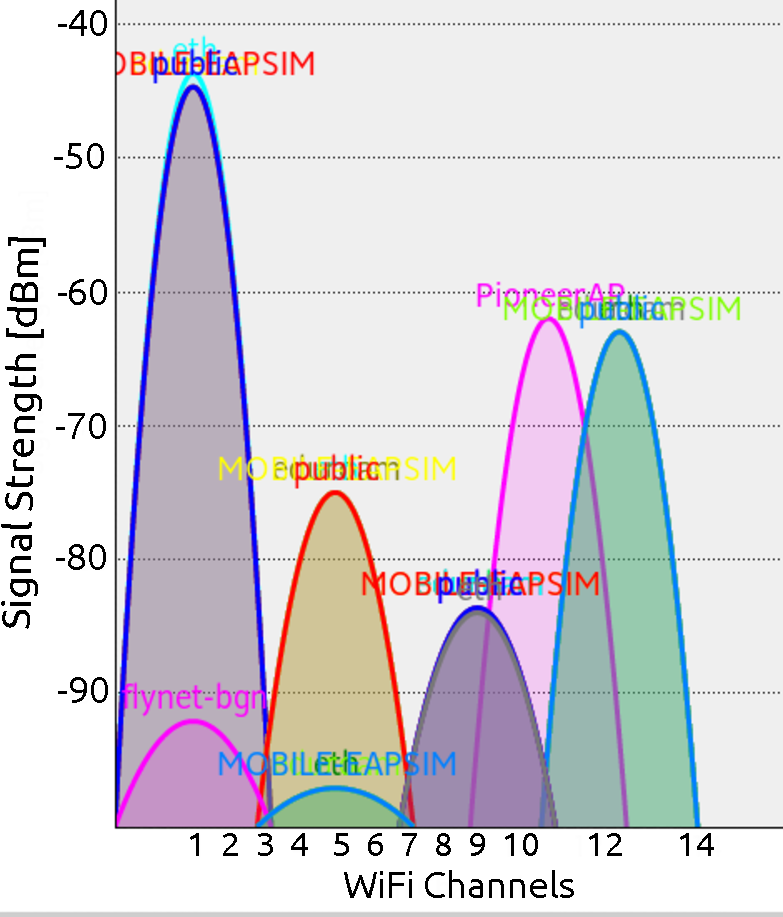
\includegraphics[width=0.45\columnwidth]{figure/levelE.pdf} 
%  \label{fig:benchmark_levelE_wifi_trace}
%}
%\caption{Benchmarking at Level E}
%\end{figure}
%
%The test area of Level E (located at ground level) is a narrow office corridor that has WiFi signals operating at
%all frequencies in the 2.4 GHz band. A WiFi trace (Fig.
%\ref{fig:benchmark_levelE_wifi_trace}) reveals a sizeable amount of WiFi
%interference at the operating frequency from a nearby access point.
%
%
%\subsection{Measurements}
%A calculation of the instantaneous Frames Per Second (FPS) was done each time
%new images were received at the server. The FPS formula used was a simple
%moving average of the $K$ most recent images ($K=5$ in our tests). In other
%words:
%
%\begin{equation}
%FPS=\left[\frac{\sum_{i=1}^K t_i}{K}\right]^{-1}
%\label{:fps}
%\end{equation}
%where $t_i$ represents the duration taken for the $i-th$ image to arrive at the
%server after the $(i-1)-th$ image. Each instantaneous FPS value obtained
%throughout the experiment was recorded.
%
%%\subsection{Results of Benchmarking}
%The instantaneous FPS values recorded at the various distances in the two
%locations were plotted to see the spread of values. The results are
%shown in Fig. \ref{fig:benchmark_boxplots}.
%
%%%% attach the Level A graphic on the left, and then Level E graphic on the right here.
%\begin{figure}
%\centering
%\subfigure[Level A]{
%%  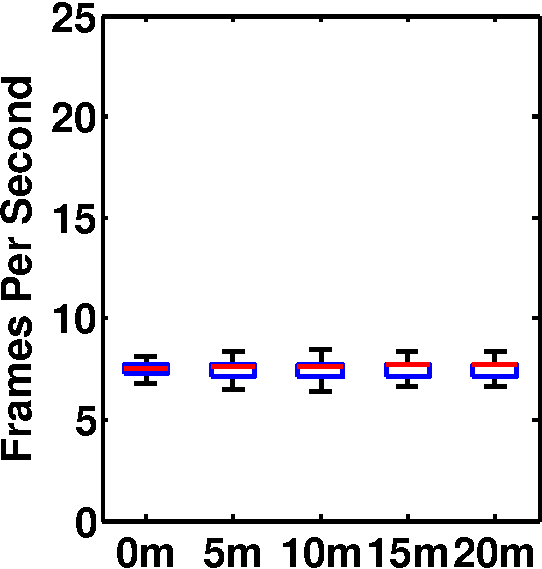
\includegraphics[height=0.45\columnwidth]{Tex_Picts/MATLAB_Figs/LevelA/Benchmark/boxplot_FPS_against_dist_levelA_notitle.pdf}
%  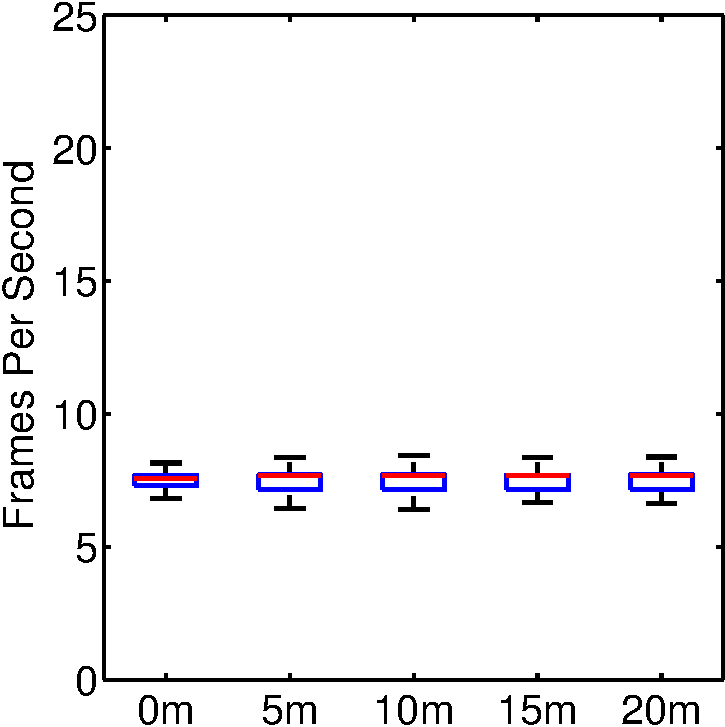
\includegraphics[height=3.7cm]{Tex_Picts/MATLAB_Figs/LevelA/Benchmark/boxplot_FPS_against_dist_levelA.pdf}
%  \label{fig:boxplot_FPS_benchmark_levelA}
%}
%%add desired spacing between images, e. g. ~, \quad, \qquad etc.
%%(or a blank line to force the subfigure onto a new line)
%\subfigure[Level E]{
%  %    \includegraphics[height=0.45\columnwidth]{Tex_Picts/MATLAB_Figs/LevelA/Benchmark/boxplots_FPS_against_dist_levelE_notitle.pdf}
%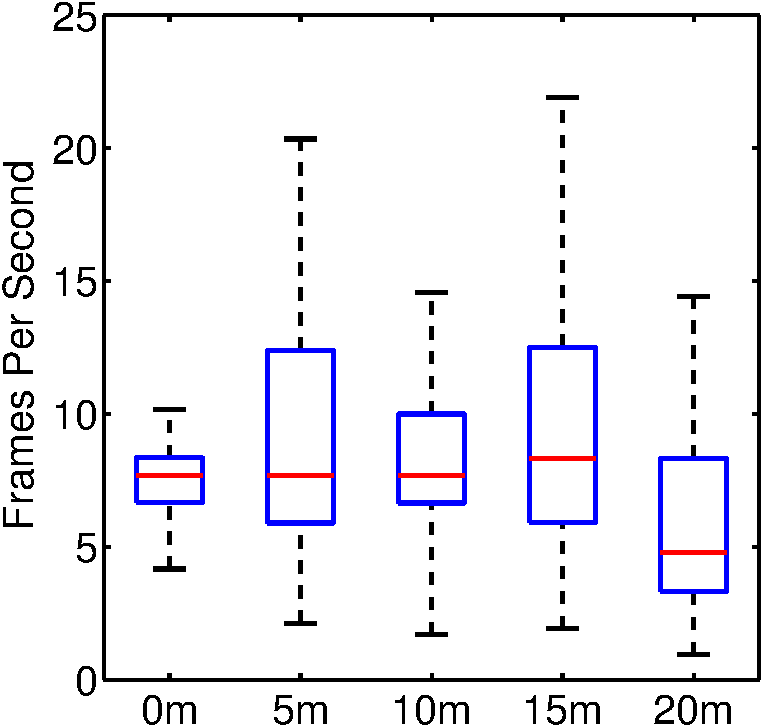
\includegraphics[height=3.7cm]{Tex_Picts/MATLAB_Figs/LevelA/Benchmark/boxplot_FPS_against_dist_levelE_notitle.pdf}
%\label{fig:boxplot_FPS_benchmark_levelE}
%    }
%\caption{Benchmarking Results}
%\label{fig:benchmark_boxplots}
%\end{figure}
%
%Figure \ref{fig:boxplot_FPS_benchmark_levelA} shows the results obtained in 
%Level A (with minimal interference). It shows that all the nodes report a similar
%FPS interval range that is between 7.56 to 7.68. This is pretty close to the
%camera frame rate of 7.5 Hz. From Fig. \ref{fig:boxplot_FPS_benchmark_levelE}
%(Level E, with significant interference), one can observe much larger ranges of FPS values
%at each distance interval. The median FPS values recorded at Level E range from
%4.78 to 8.33, which is larger (slower) than the corresponding range found at
%Level A.
%
%The larger range of FPS values seen at Level E is due to the higher amount of WiFi
%interference present along the test area. At times when the E-puck is unable to
%establish a link with the server due to interference, the data packets are
%stored in the transmission queue. 
%Consequently, no data was received at the
%server, and so the FPS value decreased. However, once the E-puck was able to
%establish a connection with the server again, the RT-WMP immediately sent these
%queued data packets out to the server as rapidly as possible.
%%(all in accordance with hard real-time rules)
%As a result, the server received these data packets
%in extremely quick succession, thus reporting an extremely high instantaneous
%FPS value at those instants.
%
%In other words, a network whose nodes yield a smaller spread of FPS values, as
%well as having a median FPS close to the frame rate of the camera source,
%corresponds to a network that is experiencing low interference and is, hence,
%performing well. This is due to the fact that all data packets that arrive at
%the transmission queue are immediately transmitted, thereby leading to a
%consistent flow of data throughout the entire network. On the other hand, a
%larger spread of FPS values and median FPS values that lie far from the frame
%rate of the camera source relates to a network whose performance is degraded,
%most likely due to significant amounts of interference. The many breaks in
%transmission result in non-uniform data flows, as packets get queued when links
%are broken and then get sent in rapid succession again when the links are
%reestablished, thereby leading to a wide range of FPS values.
%
%All these observations show that congestion in WiFi bandwidth, which is a
%typical resource in the networked robotic system, greatly affects the
%transmission quality.
%In order to achieve optimal transmission of data, a resource allocation
%strategy is necessary. The proposed strategy is discussed in the next section.

\section{RT-WMP Overview}
This section introduces the RT-WMP routing protocol and 
 the extended modification in this paper. 

\subsection{Overview}
The RT-WMP is a token-based routing protocol that works with existing IEEE
802.11 b/g/n protocols. It is chosen as the routing protocol in the ad-hoc
networks of the experiments because of its robust multi-hop capability.
Different from other ad-hoc networks, data flows in the network with
RT-WMP routing protocol could be dynamically prioritized, allowing the
user to manage the message priorities for transmission. 

The notable features of RT-WMP that contributed to its
selection are highlighted as follows:

\begin{itemize}
\item 
 Easy implementation in the user space of a Linux system;
\item
 Comparability with existing WiFi equipment;
 \item
 Storage of incoming messages in the transmission queue
of the same priority done in FIFO order;
\item
 Ability to fulfill real-time requirements.
\end{itemize}

The interested reader may refer to \cite{Danilo07rtwmp} to get more
details on the protocol and \cite{tan2013icia} to get more detail
experimental benchmarking.

\subsection{Modification of RT-WMP}
The basic RT-MMP only provides data messages management with fixed
priorities.
However, resource allocation for cloud robotic network needs dynamic
priority to adapt the task requirements and optimize the bandwidth usage. 
We have subdivided the transmission slots and implemented with
a dynamic priority mechanism. 

%\subsection{Transmission Slots Subdivision}

%The network resource is modelled as a finite queue of individual transmission
%slots, which demonstrate the limited resource in the network because each
%transmission slot can be utilized by one node in the network only.
Each transmission slot is further subdivided into four phases, namely
\textit{Auction, Priority Increase, Data Transmission} and \textit{Priority
  Reduction}, as shown in Fig. \ref{fig:conduct_of_expt_0}.
Each of these phases is explained in detail as follows:
\begin{figure}[htpb]
\centering
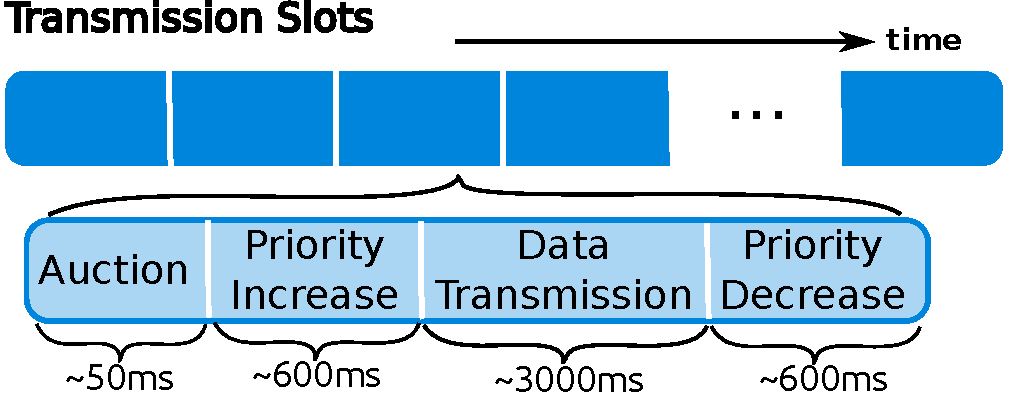
\includegraphics[width=0.9\columnwidth]{Tex_Picts/strategy_slots} 
\caption{Structure of transmission slots}
\label{fig:conduct_of_expt_0}
\end{figure}

\subsubsection{Auction}
As each transmission slot can be utilized by one node in the network only, each
node is required to bid for the transmission slot. 
%The auction follows a typical first-priced style auction, in which the winning
%bid is the highest one. 
A consensus procedure is introduced to share the individual bid of each node in
the network and find the index of the winner node with the corresponding bid.  
%The individual bid of each node is broadcast to all nodes in
%the network. The nodes then compare their own bids with the bids of the other
%nodes locally. 
Other bidders then wait for the \textit{Auction} phase of
the next transmission slot, while the winner moves on to the next phase.  
This phase lasts around 50ms in average.
Note that the detailed bidding strategy is explained in Section
\ref{sub:bidding_strategy}.

\subsubsection{Priority Increase}
The winner of the auction is authorized to increase its priority to transmit
to all the other nodes.
The duration of this phase may vary from different kind of hardware used.
For example, the E-puck robots required approximately 600ms to adjust their
priorities including token passing and bid update in our experiment. 
Thus, this phase is designed to accommodate this.

\subsubsection{Data Transmission}
The bulk of the transmission slot is dedicated to the transmission of the data
payload. For example, it is lasting 3000ms in our experiment using E-puck.

\subsubsection{Priority Decrease}
Once the \textit{Data Transmission} phase is over, the winning node's priority
is reduced to its original value. The \textit{Auction} phase of the next
transmission slot starts and the cycle then repeats itself.
As mentioned earlier, this phase is  600ms long for the
  priority changing of E-pucks'.

\section{Incremental Resource Allocation}
\label{sec:alg}
The limited network resource can be modeled as a finite queue of
individual transmission slots, which can be utilized by one node at a time
in the network only.
Therefore, this section describes the aim and the mechanism of the
developed resource allocation strategy.
\vspace{-0.3cm}
\subsection{Objective}
%The aim of the resource allocation strategy is two-fold:
%\begin{itemize}
%\item \textit{Fair Transmission}:
%For an autonomous network system, to allocate the network resource as
%fairly as possible. 
%\item \textit{Biased Transmission}:
The aim of the resource allocation strategy is \textit{Biased Transmission}:
when data from an individual node is deemed to be desired on different
priorities to the user, to allocate $P_{\text{ref}}$ \footnote{In this paper,
  we choose $P_{\text{ref}}=80\%$.} of the network resource to a particular
  node that the user wishes to favor.  
At the same time, ensuring that all other nodes still get to transmit during
the remaining $1-P_{\text{ref}}$, albeit at a lower frequency. 
%\end{itemize}
The \textit{Biased Transmission} can give some choice to the user while
ensuring that there is no large backlog of data packets stored in the
transmission queues because of a node's inability to transmit.

\subsection{Problem Formulation}
Given the objectives, we formulate the problem as the minimization of the
total cost in the following,
\begin{equation}
\begin{aligned}
\min c(t,h) = \min \sum_{i=1}^n c_i(t_i,h_i),  \\
\text{s.t.} \quad \sum_{i=1}^n t_i \leq T,  
%  1 \leq h_i(t_i) \leq H,
\label{equ:maxmin}
\end{aligned}
\end{equation}
where $c(t,h)$ is the total cost function, $c_i(t_i,h_i)$ is the cost of node
$i$, $h_i$ is the hop number of node $i$ to the server, and $T$ is the
deadline of the transmission.  
%$H$ is the largest hop number in the ad-hoc network.

%\subsubsection{Cost Function in Fair Transmission}
The cost function that considers the waiting time cost and transmission cost 
is formulated as 
\begin{equation}
c_i(t_i,h_i) = f_i(t_i) + \Delta_i(h_i),  % + \Upsilon_i(t_i) , 
\label{equ:cost}
\end{equation}
where $f_i(t_i)$ is the waiting time cost function, and $\Delta_i(h_i)$ is the
transmission cost of node $i$.
 %and the user incentive component is denoted by $\Upsilon_i(t_i)$. 
Each of these components is explained as follows. 
\begin{enumerate}
\item{Time cost $f_i(t_i)$:}

\begin{figure}
\centering
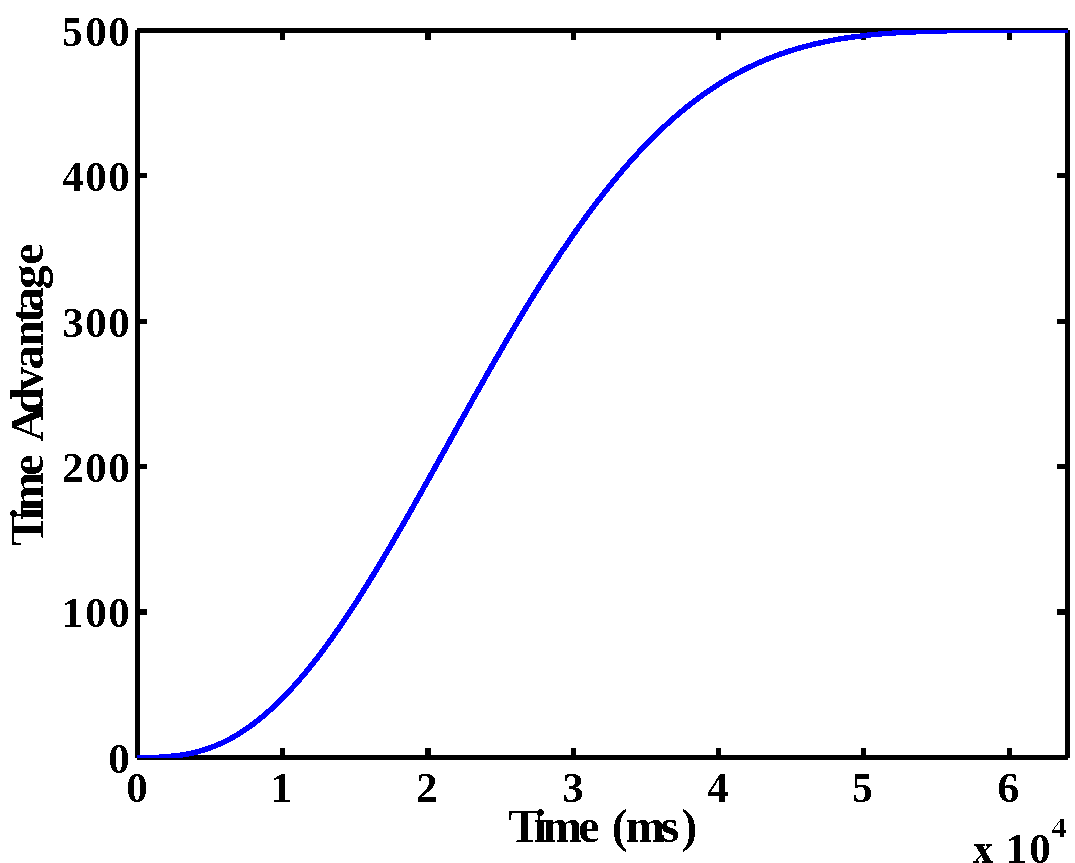
\includegraphics[width=0.7\columnwidth]{Tex_Picts/MATLAB_Figs/aging_func.pdf} 
\caption{Time cost Function $f(t)$}
\label{fig:time_advantage_func}
\end{figure}
Drawing inspiration from job scheduling literature, the aging
\cite{Rudek2012aging} is used to ensure the jobs with lower priority will
eventually complete their execution tasks. 
In this paper, a monotonically increasing function is proposed and
presented in Fig. \ref{fig:time_advantage_func}.
It depicts a typical shape for a time cost function, which can easily adapt to
other polynomial function as long as the idea is the monotonically increasing
and convergence to a value. 
Here, it is defined by a seventh-order polynomial as 
\begin{equation}
\begin{aligned}
f_i(t_i) = &1.7\times10^{-23}t_i^7-5.08\times10^{-25}t_i^6 \\
           &+5.85\times10^{-20}t_i^5 -3.12\times10^{-15}t_i^4 \\
           &+6.65\times10^{-11}t_i^3,
\end{aligned}
\end{equation}
where $t_i$ denotes the duration since the node $i$ last transmitted. 
The function has been designed to have a steep gradient so that a greater
distinction between waiting nodes can be reflected in the cost. % bids. 
In our function, to ensure that it remains bounded, the function tapers off and
eventually reaches its maximum value of 500 when $t_i = 64000$ assuming that 
one transmission with scheduling should be completed in $64000$ms.

\item  Transmission cost $\Delta_i(h_i)$:

In the ad-hoc network, each node calculates a shortest routing path and  passes
the  packets through its neighbors. 
%Most routing protocols aim to send data packets with  
% an as high as possible utilization and minimal delay. 
%This usually results in nodes nearer the server being allowed to transmit more
%frequently than other nodes that may be situated further away and require more
%hops to transmit to send their data.
%Thus, the \textit{transmission cost} formula has been modelled as  
%``assistance'' to nodes further away from the server and is given as
Thus, nodes that are further away from the server cost more regarding packet
transmission.    
The transmission cost formula is given as
\begin{equation}
\Delta_i(h_i) = a^{h_i},
\label{eqn:hop_advantage}
\end{equation} 
where $a$ is a scalar that varies with the number of nodes in the network.
It is better to determine $a$ from simulations (refer to Section
      \ref{sec:incsimulation}) since the network structure is dynamic. 
$h_i(t_i)$ is the number of hops to reach the server that affects the
transmission cost. 
\end{enumerate}

%\subsubsection{Cost Function in Biased Transmission}

%\item User incentive $\Upsilon_i(t_i)$:
%%\subsubsection{User Incentive}

\subsection{The Auction-based Mechanism}
\label{sub:bidding_strategy}

%The objective of resource allocation, the global objective is the
%total cost $c(t,h)$ and the local objective functions are $c_i(t_i,h_i)$. 
%The mapping between the global and local functions are given by the
%minimization problem (\ref{equ:maxmin}).
The problem (\ref{equ:maxmin}) should be decomposed into subtasks that
each node can perform, which is suitable to be solved by market-based
mechanisms such as auctions. 
In general, an auction is a negotiation mechanism with explicit rules that
specify how products are assigned to the winner of a number of consumers.
Especially, the cost function minimization of each node should contribute to
the cost minimization of the overall system
\cite{dias2006market,shoham2008multiagent}.
Moreover, the multi-hop network is suitable to implement a distributed
solution. 
The bidding information flow can be represented by modeling the network
communication in a dynamic graph $\mathcal{G}=(V,E,t)$, where
$V=\{v_1,v_2,\dots,v_n\}$ is the set of nodes, and $E\subset V\times V$ is the
set of edges, which indicate the link quality between nodes. 

\subsubsection{Bidding Strategy}
Suppose that each node waits time $t^{[i]} \in R^+$ for data transmission and
a period $\tau$ can wait longer or shorter.

%For \textit{Fair Transmission}, each node computes the following two bids:
For non-favored nodes, the two bids are computed by
\begin{equation}
\pi_+^{[i]} = \left\{ \begin{array}{ll}
c_i(t^{[i]}+\tau,h_i)- c_i(t^{[i]},h_i), & \text{if $t^{[i]}$ is admissible}, \\
0, & \text{otherwise},
\label{equ:bid_add}
\end{array}\right.
\end{equation}
where $\pi_+ \in R$ in (\ref{equ:bid_add}) is the injection amount that node
$i$ has to spend because of the longer waiting time $\tau$.
The bid is only related to $t_i$ because the auction mechanism is applied
before transmission. 
\begin{equation}
\pi_{-}^{[i]} = \left\{ \begin{array}{ll}
c_i(t^{[i]},h_i)- c_i(t^{[i]}-\tau,h_i), & \text{if $t^{[i]}$ is admissible}, \\
0, & \text{otherwise}, 
\label{equ:bid_minus}
\end{array} \right.
\end{equation}
where $\pi_{-} \in R$ in (\ref{equ:bid_minus}) is the suppression amount that
node $i$ can save because of the less waiting $\tau$. 
%
%The basic bidding algorithm relies on the discretized step $\tau$ for
%searching the optimal value.
%The algorithm may only derive the local optimal value regarding of the
%selection of discretized step $\tau$.
%Therefore, we add a \textit{user incentive} $\Upsilon_i$ in bidding to provide
%multiple selections of discretized step beside $\tau$ for \textit{Biased
%  Transmission}. 
 
%For \textit{Biased Transmission},
For the favored node, the \textit{user incentive} $\Upsilon_i$ is added to the
bid.
It simply elevates the favored node's cost above all the other nodes, thereby
allowing that node to bid more and hence have won more transmission slots.
However, this incentive cannot remain at its current value as none of the
other nodes would be able to transmit.  Thus, a ``decrease-and-replenish''
system is utilized to adjust continuously the incentive of the node, which is
described below with the aid of Fig. \ref{fig:incentive}. 
\begin{figure}[htpb]
\centering
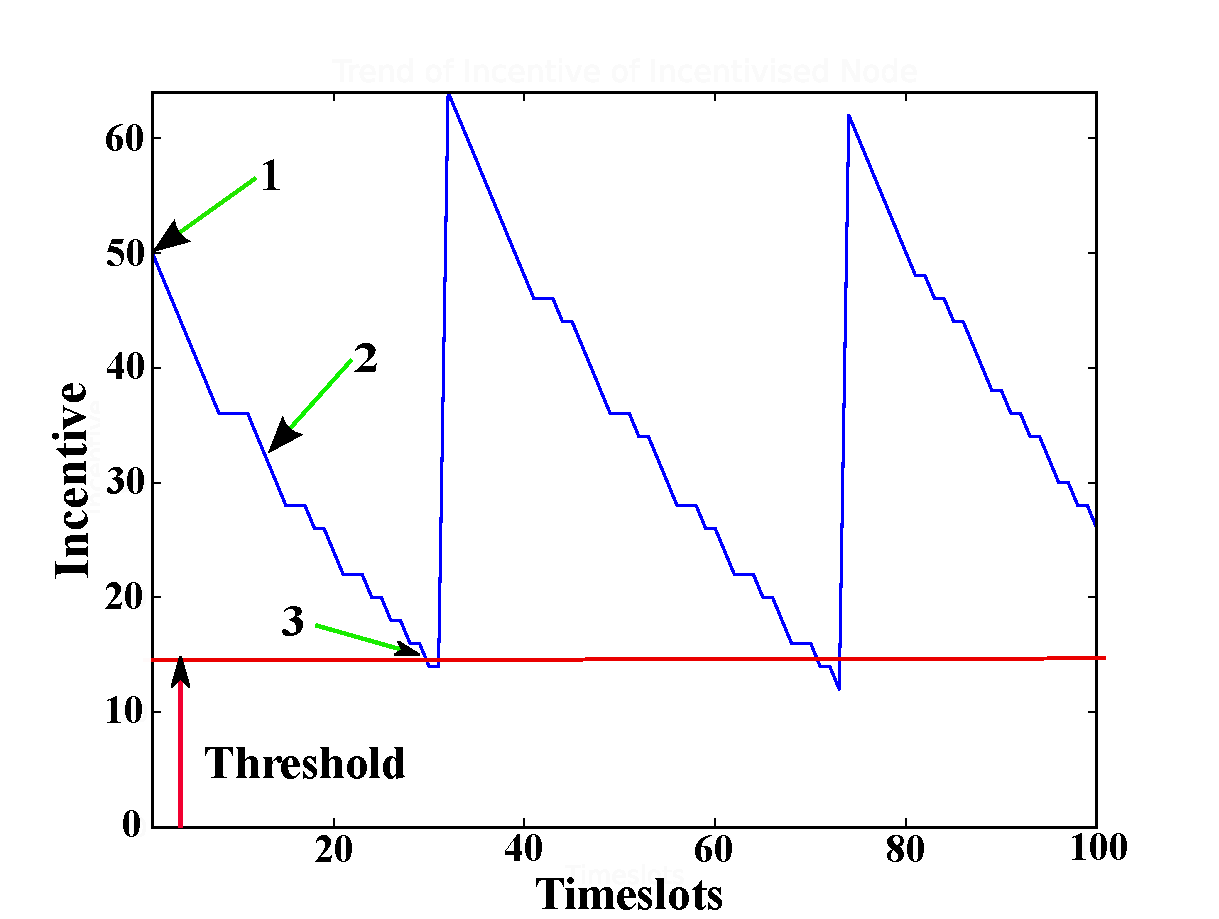
\includegraphics[width=0.8\columnwidth]{Tex_Picts/incentive_trend_annotated-crop.pdf} 
\caption{Trend of the user incentive for a favored node}
\label{fig:incentive}
\end{figure}

Assume that $t^{[i]}$ is admissible, the bids of the favored node $\hat{i}$ are
calculated as follows:
\begin{equation}
 \pi_{+}^{[\hat{i}]} = c_i(t^{[i]}+\tau,h_i)- c_i(t^{[i]},h_i),  \\
%\pi_{+}^{[\hat{i}]} = 0,  
\label{equ:favor_bid_add}
\end{equation}
\begin{equation}
\pi_-^{[\hat{i}]} = c_i(t^{[\hat{i}]},h_i)- c_i(t^{[\hat{i}]}-\tau,h_i) + \Upsilon_i, 
\label{equ:favor_bid_minus}
\end{equation}
where 
 $\pi_{+}^{[\hat{i}]}$ in (\ref{equ:favor_bid_add}) is the 
suppression bid that node $i$ can save for waiting longer time $\tau$, 
$\pi_- \in R$ in (\ref{equ:favor_bid_minus}) is the 
injection bid that node $i$ has to spend for saving the waiting time $\tau$.
%The favored node cannot wait longer for this case, so $\pi_+^{[\hat{i}]} = 0$. 

There are three cases for calculating the user incentive $\Upsilon_i$ by the
favored node $\hat{i}$. 
\begin{itemize}
\item (Arrow 1) In the beginning, the favored
node is given a certain amount of user incentive $\xi$, 
  %   which is the amount of incentive ``injected'' to node $i$,
  named ``Injection Incentive'' (refer to Section \ref{sec:incsimulation} for
        the derivation of this value).
\begin{equation}
\Upsilon_i = \xi. 
\label{eqn:user_incentive}
\end{equation}
%In other words, once the node is favored, the \textit{user incentive} is given
%as
\item (Arrow 2) When the favored node wins an auction,  
  the amount of user incentive for the favored node at the
next timestamp $k+1$ is decreased by an amount $\upsilon$,
named ``Suppression Incentive'' (refer to Section \ref{sec:incsimulation} for
  the derivation of this value).
%In other words, for each iteration where the
%node wins the auction, it calculates the bid as: 
%\begin{equation}
%\pi_+^{[\hat{i}]} = c_i(t^{[i]}+\tau_-)- c_i(t^{[i]} - \upsilon
%\label{equ:favor_bid_add_1}
%\end{equation}
%where $\pi_+ \in R$ in (\ref{equ:favor_bid_add_1}) is the suppression amount that
%node $i$ can save for longer waiting time $\tau_+$.
%\begin{equation}
%\pi_{-}^{[\hat{i}]} = 0,  
%\label{equ:favor_bid_minus_1}
%\end{equation}
%\textit{user incentive} is now 
\begin{equation}
\Upsilon_i[k+1] = \Upsilon_i[k] - \upsilon.
\label{eqn:incentive_decrease}
\end{equation}
Then the total bid of the favored node decreases over time, thereby
allowing the other nodes the chance to win the auction and transmit.
Note that if the favored node does not win a particular auction, then the 
user incentive is not decreased.
	
\item (Arrow 3) Once the amount of user incentive decreases to a
certain threshold value, it is immediately replenished with $\xi$.
Mathematically, it is given by
\begin{equation}
\label{equation:user_injection}
\Upsilon_{i}[k+1] = \Upsilon_{i}[k] + \xi.
\end{equation}
This replenishment allows the favored node to win more of the following
auctions, thereby ensuring that it gets to transmit for $P_{\text{ref}}$ of the
time.
\end{itemize}
%Each node $i$ in the network follows the same bidding strategy. For a
%\textit{Fair Transmission} at some transmission slot $t_i \in \mathbb{Z}$,
%  the bid $B$ is defined as follows,
%
%\begin{equation}
%B_i(t_i)=f_{i}(t_i) + \Delta_{i}(t_i),
%\label{equ:bid_fair}
%\end{equation}
%where the user incentive $\Upsilon_i(t_i) = 0$.
%For a \textit{Biased Transmission}, the user incentive component, denoted by
%$\Upsilon_i^t$, is included. The bid is 
%\begin{equation}
%B_{i}(t_i)=f_{i}(t_i)+ \Delta_{i}(t_i) + \Upsilon_i(t_i).
%\label{equ:bid_biased}
%\end{equation}

\subsubsection{Consensus Procedure}
%Each node $i$ uses the defined bid in (\ref{equ:bid_add}) and
%(\ref{equ:bid_minus}) in the auction procedure.
Each node $i$ initializes the information of the bid and its node index
as $\{x^{[i]},y^{[i]}\}$, where the bid is calculated by
(\ref{equ:bid_add}) and (\ref{equ:bid_minus}).
Because of the multi-hop network graph $\mathcal{G}$ infrastructure, each node
only directly communicates with neighbors at each time instant $k$, the
nodes perform a consensus procedure on the highest bid and the corresponding
node index.  
Then, nodes update the index and bid of current auction winner as follows,
\begin{eqnarray}
x^{[i]}[k+1] = \max_{j\in \mathcal{N}_i \cup \{i\}} (x^{[j]}[k]), \\
\label{equ:bid_value_update}
y^{[i]}[k+1] = y^{[j^*]}[k], \\
\label{equ:bid_index_update}
\text{where} \quad
j^* = \argmax_{j\in \mathcal{N}_i \cup \{i\}} (x^{[j]}[k]),
\label{equ:bid_index}
\end{eqnarray}
where $\mathcal{N}_i$ is the set of node $i$ neighbors.
Each node saves the highest value and the corresponding node index among its
neighbors as in above equations. 
Therefore, the nodes reach a consensus on the highest bid $\pi_+^*$ from node
$i^*$ and $\pi_-^*$ from node $j^*$ within a number of iterations of nodes
in the network graph $\mathcal{G}$. 
Please note that the number of iterations needs to bid on the entire
network is equal to the communication graph diameter that is the maximum
distances connects between any two nodes.  
In practical applications, if the graph diameter is unknown, it can be
conservatively chosen as $n-1$ given an $n$-node graph. 

\subsubsection{Auction Mechanism}
After the consensus procedure, each node evaluates the difference $\theta =
\pi_-^*-\pi_+^*$.
If $\theta > 0$, $\pi_+^* >0$ and $\pi_-^* >0$, the exchanging of a period
waiting time $\tau$ between node $i^*$ and $j^*$ leads to saving $\theta$. 
Then, these nodes update their waiting time as 
%node $i^*$ is recognized as the winner, and its
%waiting time can be updated as 
\begin{equation}
t^{[i^*]} \leftarrow t^{[i^*]}+\tau, \quad t^{[j^*]} \leftarrow t^{[j^*]}- \tau. 
\label{equ:t_update}
\end{equation}
The consensus procedure ensures that the node pair $(i^*,j^*)$ provides the
global minimum cost when the waiting time is exchanging as (\ref{equ:t_update})
    is performed. 
The mechanism iterates through the above-presented step \textit{1)-3)} can lead
to a lower-cost solution. Note that the update of waiting time does not change
the amount of allocated transmission time slots. 
It is because the mechanism starts from a solution fulfilling the deadline 
constraint $\sum_{i=i}^n \leq T$, which is always accommodated during the 
auction-based mechanism.


\section{Simulations}
\label{sec:incsimulation}
Simulations were required to determine suitable parameters for the following
variables:
\begin{itemize}
%\item $Minimum\, Bid$
\item Hop scalar: $a$ defined in  (\ref{eqn:hop_advantage}),
\item Injection incentive % $\pi_+$ defined in (\ref{equ:bid_add}), 
  defined in equation (\ref{eqn:user_incentive}),
\item Suppression incentive % $\pi_-$ defined in (\ref{equ:bid_minus}).  
  defined in equation (\ref{eqn:incentive_decrease}).
\end{itemize}
The simulations conducted are subject to the same simulation environment. 
The topology used for simulation is a string topology, where nodes have to send
data back to a server by hopping through other nodes along the string. 
A system utility function is also defined to measure the goodness of the
simulation results.

\subsection{System Utility Function}
The aim of the system utility function is to determine how close the
simulation results are towards achieving the aim of the resource allocation
strategy.
%This utility function is later implemented in the actual setup to track and
%reveal the status of the network.
The system utility function is $U(t)$, where
%\begin{align}
%%\begin{eqnarray}
%%\begin{split}
%U(t) = \lambda \left(U_{1}(t) \right) + (1-\lambda)\left(U_{2}(t)\right),\\
%\begin{cases}
%\lambda = 0,\quad  \textit{for Fair Transmission}; \nonumber \\
%\lambda = 1,\quad  \textit{for Biased Transmission}; \nonumber
%\end{cases} 
%%\end{split}
%\end{align}
%%\end{eqnarray}
%%\end{ation}
%%\[
%%  \left\{\begin{array}{{l{\quad}l}
%%  %\left\{\begin{array}{@{l@{\quad}l}
%%$\lambda = 0$, & \mbox{if $y=1$} \\[\jot]
%%$ \lambda = 1$, & \mbox{if $b=2$}
%%      \end{array}\right.
%%  \]}
%where $U_{1}(t)$ and $U_{2}(t)$ are the sub-utility functions that determine how
%close the network is to the ideal for the \textit{Biased Transmission} case and
%\textit{Fair Transmission} case respectively at a particular instant. 
%In addition, 
\begin{equation}
\centering
0 \leq U(t) \leq 1,
\end{equation}
if $U(t) = 1$ denotes an ideal network.
Thus, the goal of the resource allocation strategy is to ensure that $U(t)
  \rightarrow 1$ as much as possible.
Each of the sub-utility functions is described in detail as follows.

%\subsubsection{Sub-utility Function for Biased Transmissions, $U_{1}(t)$}
%\label{subsub:utility_func_biased_transmissions}
Past recent transmission instants are taken as sources to compute the utility
function.
The reference number of transmission slots is:
\begin{equation}
\centering
R_f = \beta n,
\label{equ:R_f}
\end{equation}
where $n$ is the number of nodes in the network and $\beta$ is a coefficient
  of transmission slots.  We empirically choose $\beta=3$,
which means three times the number of the nodes as a reference amount
of transmission slots. 
From the past number of transmission, $P_{f}$, the proportion of the number of
transmission slots taken up by the favored node, can be calculated as
\begin{equation}
P_{f}(t)=\frac{S_{f}(t)}{R_f},
\label{equ:P_f}
\end{equation}
where $S_{f}(t)$ is the number of transmission slots taken up by the favored
  node at time instant $t$.

Next, recalling that the favored node is only allowed to transmit for
$P_{\text{ref}}$ of the transmission slots.
The utility value is one when it corresponds to an ideal network, 
%The utility value corresponds to an ideal network is one, 
%An ideal network corresponds to a utility value to 1, 
and then the utility function %for \textit{Biased Transmissions} 
can be defined as
\begin{equation}
U(t)= e^{-\mid P_{f}(t) - P_{\text{ref}}\mid}.
\end{equation}
Therefore, whenever the favored node does not transmit $P_{\text{ref}}$ of the
  time, $U(t)<1$.
  %the utility function will reflect this by returning a value less than 1.

%\subsubsection{Sub-utility Function for Fair Transmission, $U_{2}(t)$}
%We use the same past $R_f$ transmission slots for \textit{Fair Transmission} as
%  defined in equation (\ref{equ:R_f}). %for \textit{Biased Transmissions}.
%%  in Section \ref{subsub:utility_func_biased_transmissions},
%The mean number of transmissions slots taken up by each node, $\bar{s}(t)
%  = \frac{1}{n} \sum_{i=1}^n S_{fi}(t)$, is calculated, where $S_{fi}(t)$ is
%  the number of transmission slots used by the $i$-th node at time $t$.
%%and $\bar{t}$ is the average time of the transmission slots.
%Then, the mean squared error, $\varepsilon$, and standard deviation, $\sigma$
%are calculated as 
%%\[
%\begin{equation}
%\begin{aligned}
%&\varepsilon(t) = \frac{1}{n} \sum\limits_{i=1}^n (S_{fi}(t) - \bar{s}(t))^2, \\
%&\sigma(t) = \sqrt{\frac{n}{n-1}\varepsilon(t)}.
%\end{aligned}
%\label{equ:mse}
%\end{equation}
%%\]
%The standard deviation gives a good measure of the fairness of the network,
%because if $\sigma(t) = 0$, then the nodes are transmitting fairly;
%on the other hand, if $\sigma(t) \neq	0$, then there is some amount of
%unfairness in the network.
%In order to express the amount of fairness as the sub-utility function for this
%transmission case, % the $\sigma(t)$ variable is treated as 
%the sub-utility function for \textit{Fair Transmission} can be defined as
%\begin{equation}
%U_{2}(t) = e^{-\sigma(t)}.
%  \label{equ:sd}
%\end{equation}
%Hence, when the network is fair, $U_{2}(t) = 1$; otherwise, $U_{2}(t) < 1$.

%\subsection{Simulation Environment}
%The topology used for simulation is a string topology, where nodes
%have to send data back to a server by hopping through other nodes along the
%string. 

\subsection{Selection of Cost Function Parameters}
Hop Scalar $a$ is the first to be determined by a various number of nodes.
It is selected by assuming the user incentive $\Upsilon=0$ and executing 500
transmission slots  
%under a \textit{Fair Transmission}
 for $0.5 < a < 50$. 
Once $a$ is selected, the remaining two parameters, Injection Incentive
$\xi$ and Suppression Incentive $\upsilon$ are selected by running 500
transmission slots under a \textit{Biased Transmission} case.
All selections are chosen based on the outcomes that give the highest utility.
Table \ref{tab:chosen_variable_values} gives the chosen values that are finally
used in the algorithm.

\newcolumntype{L}{>{\centering\arraybackslash}m{1.6cm}}
\begin{table}[htpb]
  \small
\caption{Table of Parameters with Chosen Values for Various Number of Nodes}
\label{tab:chosen_variable_values}
\begin{center}
%\begin{tabular}{cccc}
%\begin{tabular}{cccc}
%\begin{tabular}{m{3.6cm}m{2cm}LL}
\begin{tabular}{m{2.3cm}m{1cm}LL}
\toprule
\centering Number of Nodes (excl. Proxy) & \centering{Hop} Scalar $a$ & Injection
Incentive $\xi$ & Suppression Incentive $\upsilon$\\ 
\midrule
\centering 2 & \centering 2.5 & \centering 50 &  25 \\ 
\centering 3 & \centering 2.0 & \centering 105 &  90 \\ 
\centering 4 & \centering 1.5 & \centering 120 &  90 \\ 
\centering 5 & \centering 1.5 & \centering 125 &  110 \\ 
\centering 6 & \centering 1.5 & \centering 155 &  125 \\ 
\bottomrule
\end{tabular} 
\end{center}
\end{table}


\section{Experiments and Validation}
\label{sec:inc_experiment}
This section first presents a brief overview the protocol applied the proposed
  algorithm. Then the effectiveness of the auction-based resource allocation
  strategy is validated by experiments, followed by discussion.

The infrastructure and function of Real Time - Wireless Multi-Hop Protocol
(RT-WMP) is suitable for our proposed mechanism.  RT-WMP can implement the
auction-based mechanism, thereby validate its effectiveness.
Some algorithms like genetic algorithm \cite{GA2011RA} have central controller
requires a high bandwidth communication that can not be implemented in the
ad-hoc network structure.
Others works assume perfect transmission \cite{ZavlDistAuc2008,Shao2014RRA} 
such as the variation of networks is homogeneous for different links.
Practically, it is not the case, we considered the dynamic change of
bandwidth, and validate the mechanism in a real ad-hoc network. 
%\cite{Zhang2014priorityRA}
Additionally, the time cost of negotiation of the resource allocation 
 is considered in our strategy design and implementation. 
Therefore, the effectiveness of the proposed strategy is convincing with
real-time ad-hoc network experiments. 


\subsection{RT-WMP Implementation}
\label{sec:rtwmp}
%We briefly reveal the implementation of RT-WMP and on the hardware
%  used.
%\subsubsection{Overview of RT-WMP} \label{subsection:overview_RT-WMP} 
%The RT-WMP is a token-based routing protocol that works on existing IEEE
%802.11bgn protocols. It was chosen as the routing protocol to be used in the
%ad-hoc networks established in the upcoming experiments because of its
%multi-hop capability. In other words, the protocol is able to route data to a
%destination node that may be out of range from the sender by hopping through
%other nodes that are within range of the sender. Furthermore, the protocol is
%able to prioritise data flows in the network dynamically. This feature was used
%heavily as part of the strategy to determine which node could transmit at any
%given time. 
%
%In addition to this useful feature, some other features that contributed to its
%selection are highlighted below:
%
%\begin{itemize}
%\item easy implementation in user space for Linux system;
%\item consequently, existing WiFi equipment could still be used;
%\item storage of incoming messages of the same priority in FIFO order
%(transmission queue);
%\item ability to fulfill firm real-time requirements.
%\end{itemize}
%
%The interested reader may refer to \cite{Danilo07rtwmp} to get a detailed
%understanding on how the protocol works.

%\subsubsection{Implementation on Hardware}
The RT-WMP protocol was implemented on seven devices in this paper, including a
server, four TurtleBot \footnote{https://www.willowgarage.com/turtlebot} with
Intel CPUs and two E-puck robots \footnote{http://www.gctronic.com/e-puck.php}
equipped with ARM CPUs.
Ubuntu and Robot Operating System (ROS) are available on these test devices.
The implementation is thus significantly simplified, as the protocol
is encapsulated in a ROS package \texttt{ros-rt-wmp}
\footnote{http://www.ros.org/wiki/ros-rt-wmp}. 
Data stream can be then transmitted among the devices as ROS topics.
Note that, as a prerequisite, an IEEE 802.11 ad-hoc network has to be
established beforehand, since the RT-WMP operates dependently on this
infrastructure.
The communication topology among the seven nodes is illustrated as Fig.
\ref{fig:rosgraph}, where
six robots transmit image topics to the server in RT-WMP protocols.
Besides, \ref{fig:connection_topology} gives an instant  network connection
topology. For example,  R4 can connect to R0 through R1 since R4-to-R1 has
higher link quality than R4-to-R2's. 

\begin{figure}[htpb]
\begin{center}
\subfigure[Communication topology of ROS topics]{
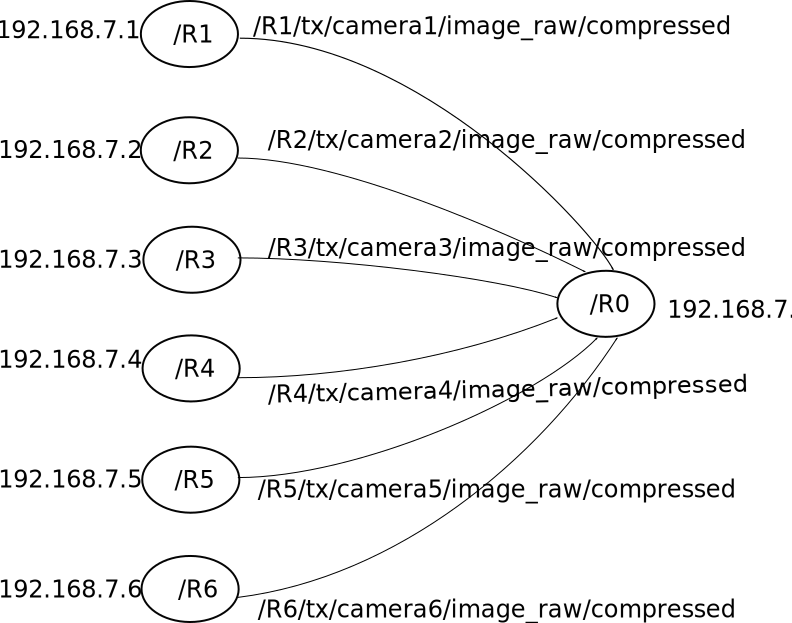
\includegraphics[width=0.9\columnwidth]{figure/rosgraph}
\label{fig:rosgraph}}
\subfigure[An instant network connection topology]{
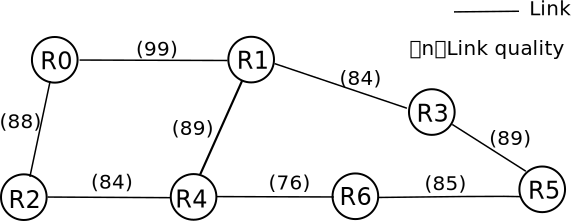
\includegraphics[width=0.7\columnwidth]{figure/hop_topology}
\label{fig:connection_topology}}
\caption{Node topology in the ad-hoc network}
\label{fig:topology}
\end{center}
\end{figure}
%%% COMMENT: Perhaps can talk about problem with the RSSI readings in the 
%%% epuck driver, but only if there is nothing else to talk about.



\subsection{Experiment Setup}
Experiments for 
 % both \textit{Fair Transmission} and 
\textit{Biased Transmission} are conducted with and without the resource
allocation strategy in order to gauge the performance improvements. 
Besides, each case is also tested with three-node and six-node scenarios, to
evaluate how the strategy behaves with an increased load.

\subsubsection{Devices Used}
Devices as various roles in the experiments are as shown in
Table \ref{tab:nodes_config}. All of them have \texttt{ros-rt-wmp} nodes
run in the user space, and the WiFi modules are operating at 2.462 GHz.

%\begin{table*}
%\centering
%\begin{tabular}{p{2.5cm}|p{0.8\textwidth}}
%\toprule
%    Server Node \protect\newline R0 & 	The proxy used is an Intel-based
%    laptop running Linux Ubuntu 12.04 LTS. It utilises a built-in Ultimate N
%    WiFi Link 5300 network card from Intel Corp, capable of running IEEE
%    802.11b/g/n. The transmission power used is set at 15dBm, the maximum
%    possible value. The proxy is configured to only receive image topics from
%    all other nodes.\\ \midrule
%
%Transmitting Node \newline R1 &  This role is fulfilled by another Intel-based
%laptop with similar specifications to the proxy, except that the transmission
%power is set at 16dBm. The built-in camera is configured to capture images at
%a frame rate of 7.0 Hz. These were then sent to R0 as compressed JPEG images
%via ROS, taking up a bandwidth of approximately 20 KB/s. \\ \midrule
%
%Transmitting Nodes \newline R2 \& R3 &  These two roles are fulfilled by the
%ARM-based E-pucks running a lean version of Linux Ubuntu 10.10 LTS. The WiFi
%dongles used are configured to run in the IEEE 802.11b/g mode. The
%transmission power is set at $15 \pm 1.5 dBm$. Each E-puck had a Point Grey
%Firefly Camera configured to capture images at a frame rate of 7.5 Hz. These
%images is then sent as compressed JPEG images over ROS. The bandwidth taken
%up by these images is approximately 30 KB/s.\\
%\bottomrule
%\end{tabular}
%\caption{Nodes involved in the tests}
%\label{tab:nodes}
%\end{table*}

%-------------------------------------------------------
% Table
%-------------------------------------------------------
\begin{table*}[htpb]
\small
\caption{Configuration of Nodes Involved in the Experiments}
\label{tab:nodes_config}
\centering
\begin{tabular}{p{0.15\textwidth}p{0.15\textwidth}p{0.25\textwidth}p{0.1\textwidth}p{0.28\textwidth}}
\toprule
\multirow{2}{*}{\text{Nodes}} & \multicolumn{3}{c}{\text{System Configuration}} &
Transmission Data\\
\cmidrule(r){2-5}
 & System & WiFi Device & Max Transmission Power & Video Sequence \\
\midrule
Proxy Node  \newline{R0} \newline{(Receiver)} & Intel-based laptop running Linux Ubuntu 12.04 LTS 
& A built-in Centrino Advanced-N 6205 wireless network card running IEEE 802.11b/g/n 
& 15 dBm & Receiving request topics from all other \newline{nodes}\\
\midrule
Transmitting Nodes \newline{R1 and R2} \newline{(Sender)}
& ARM-based E-puck running a lean version of Linux Ubuntu 10.10 LTS
& A WiFi dongle running IEEE 802.11b/g mode & $15 \pm 1.5 dBm$
%& Hundred bytes data sent via ROS at a rate of 1.0 Hz
& $\bullet$ Images of $160\times120$ pixels sent via ROS at a frame rate of 7.5 Hz
\newline{$\bullet$ 17.58 KB/s of bandwidth taken up} \\
\midrule
Transmitting Nodes R3, R4, R5 and R6 (Sender) 
& Intel-based laptops running Linux Ubuntu 12.04 LTS
& A built-in TL8188CE wireless network card running IEEE 802.11b/g/n & 15 dBm
%& Hundred bytes data sent via ROS at a rate of 1.0 Hz
& $\bullet$ Images of $160\times120$ pixels sent via ROS at a frame rate of 7.5 Hz
\newline{$\bullet$ 17.58 KB/s bandwidth taken up} \\
    \bottomrule
\end{tabular}
\end{table*}

\subsubsection{Placement of Nodes}
The experiments were carried out in open areas on two stocks of a building,
    i.e. Level A and Level E, 
where the surroundings have different conditions of interference on the WiFi channels.
It mimics different environmental conditions.
As shown in Fig. \ref{fig:wifi_trace}, the test area of Level A is a wide open
area, mainly surrounded by concrete walls. 
 A simple WiFi sweep was conducted, and the trace revealed that there were no
 other WiFi signals present at the desired operating frequency 2.462GHz
 (Channel 11) (see Fig.  \ref{fig:benchmark_levelA_wifi_trace}).
WiFi interference is thus expected to be minimal in this area.
The test area of Level E is a narrow office corridor that has WiFi signals
operating at all frequencies in the 2.4 GHz band. 
A WiFi trace (see Fig.  \ref{fig:benchmark_levelE_wifi_trace}) reveals a considerable
amount of WiFi interference at the operating frequency from a nearby
access point.

%-------------------------------------------------------
% Figure
\begin{figure}
\centering
\subfigure[Level A]{
  %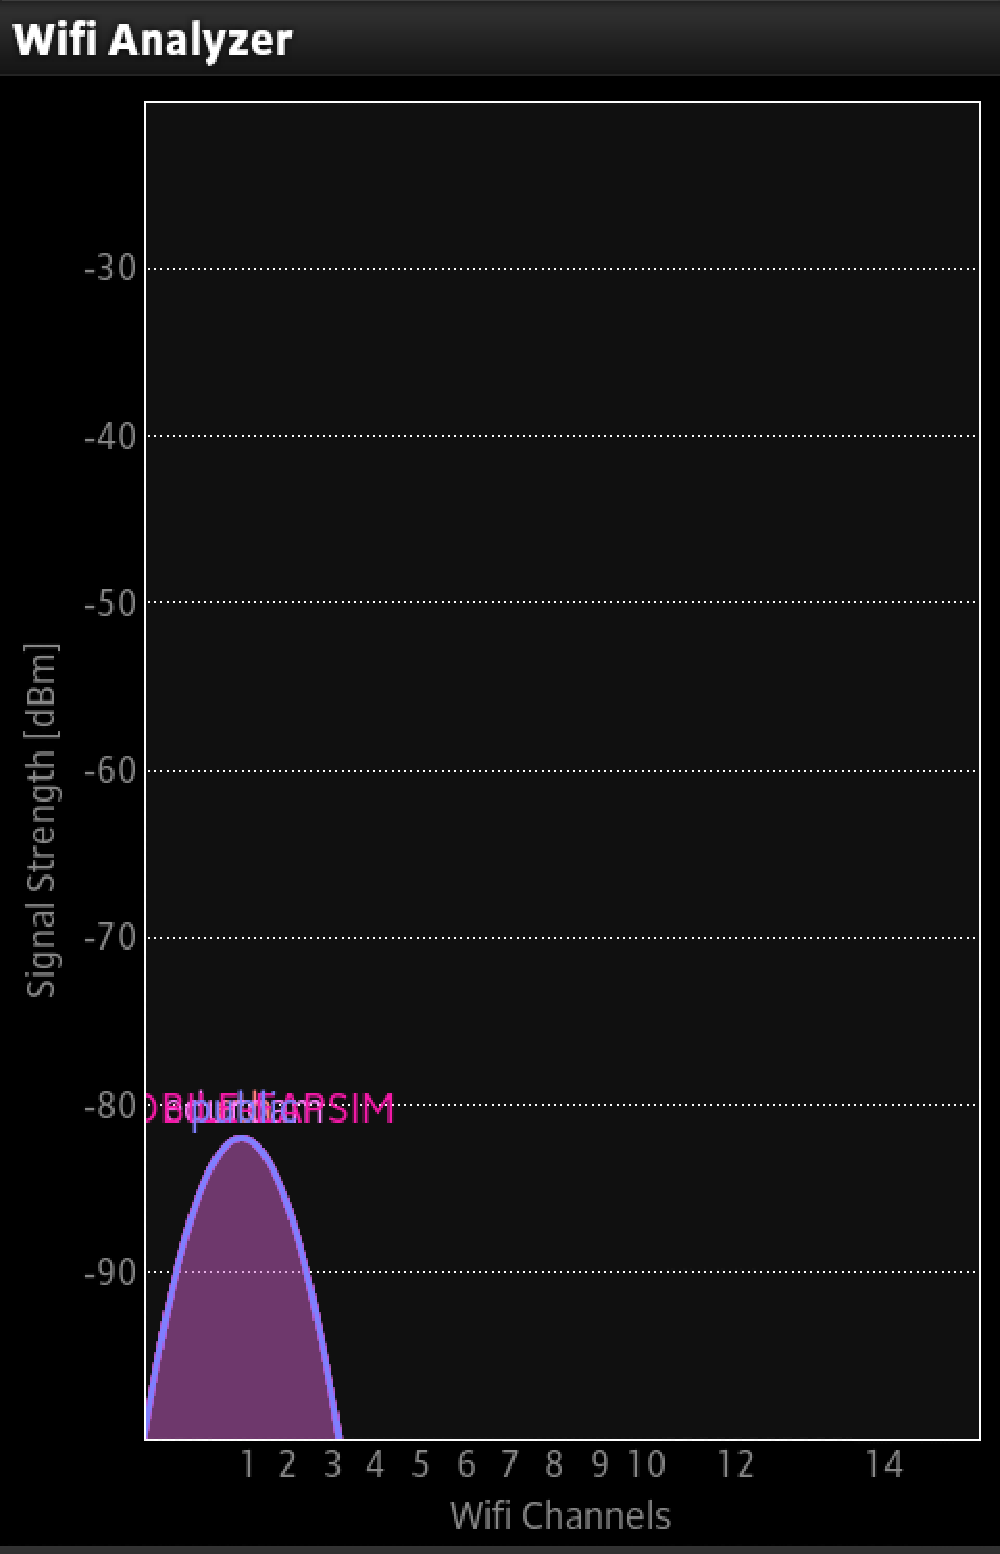
\includegraphics[width=0.22\textwidth]{Tex_Picts/levelA_edited.pdf}
  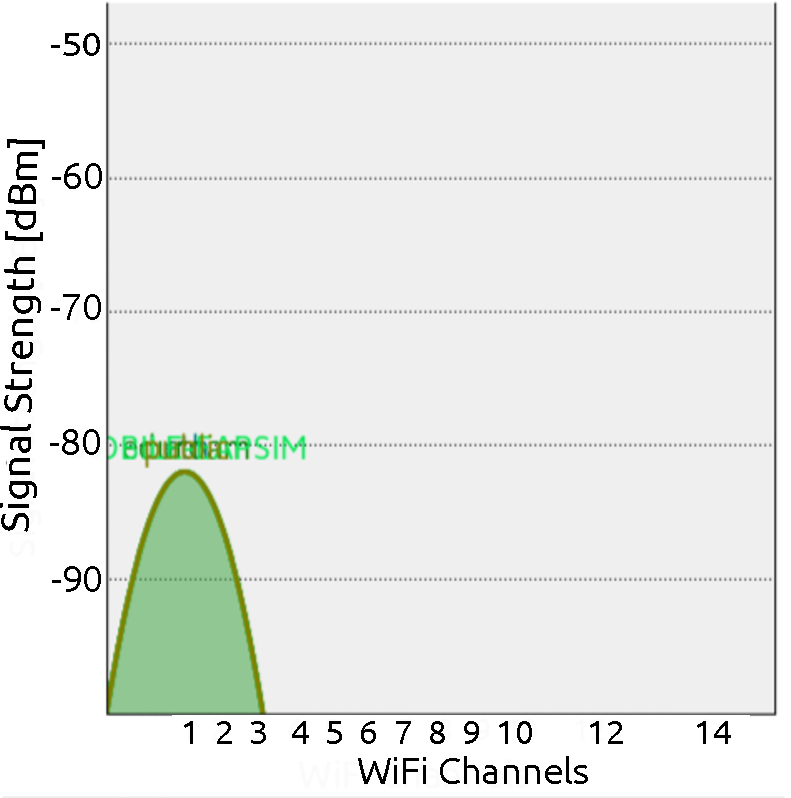
\includegraphics[width=0.46\columnwidth]{figure/levelA.pdf} 
  \label{fig:benchmark_levelA_wifi_trace}}
\subfigure[Level E]{
  %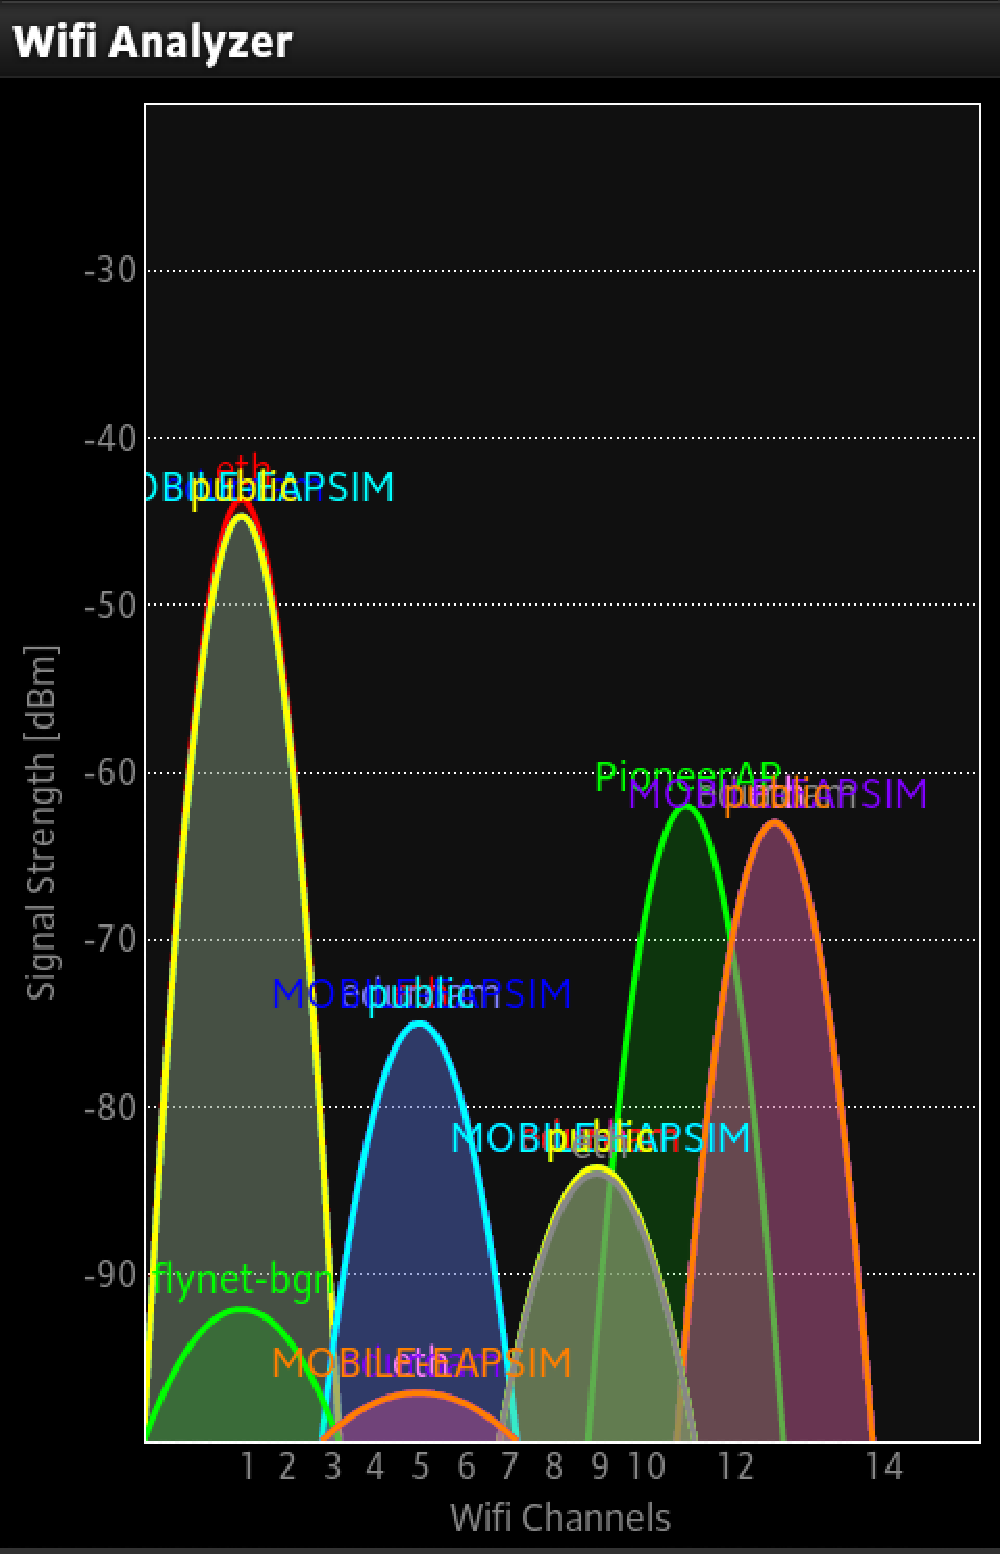
\includegraphics[width=0.22\textwidth]{Tex_Picts/levelE_edited.pdf}
  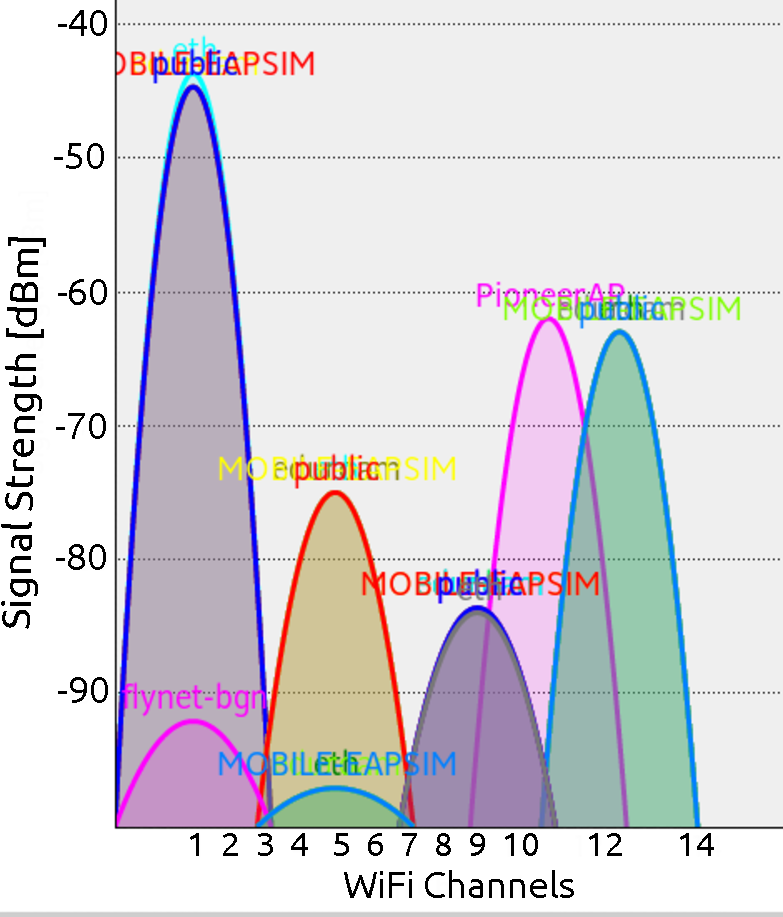
\includegraphics[width=0.45\columnwidth]{figure/levelE.pdf} 
  \label{fig:benchmark_levelE_wifi_trace}}
\caption{WiFi trace}
\label{fig:wifi_trace}
\end{figure}
%-------------------------------------------------------
\begin{figure}[htpb]
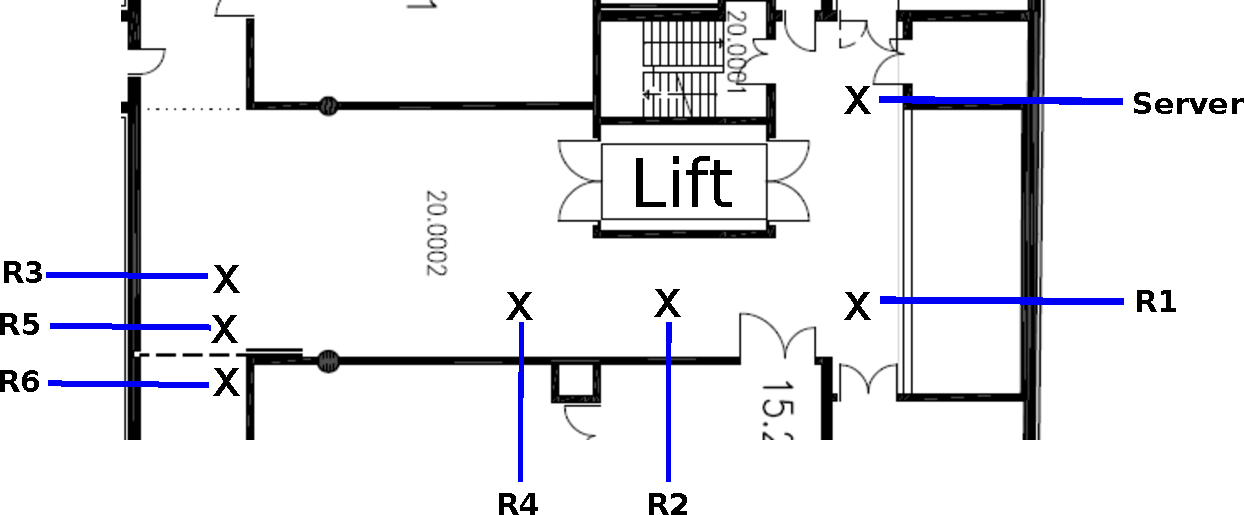
\includegraphics[width=\columnwidth]{Tex_Picts/extracted_floorplan_lujia.pdf} 
%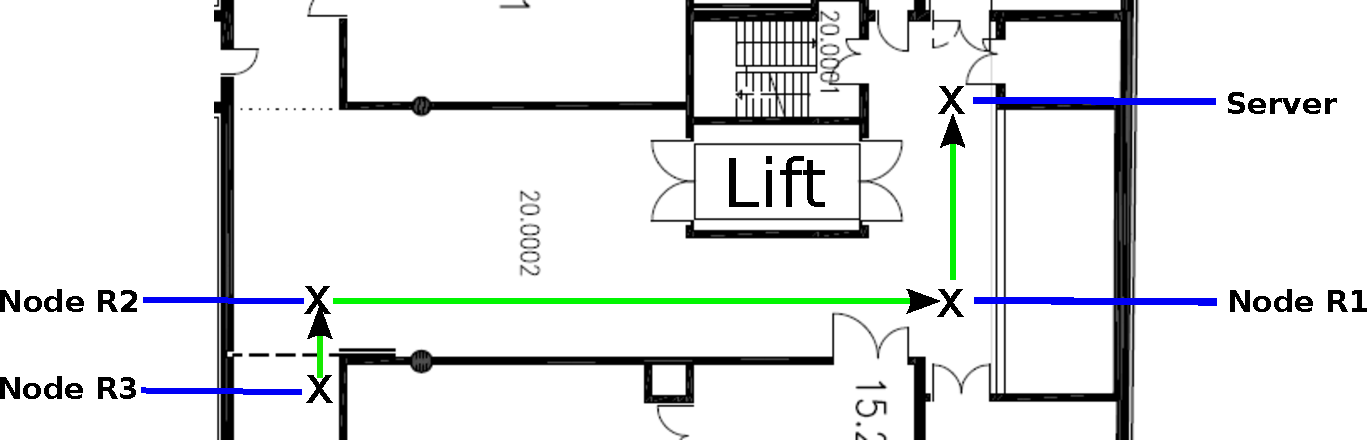
\includegraphics[width=\columnwidth]{Tex_Picts/extracted_floorplan_CLA_A_expt.pdf} 
\caption{Placement of Nodes on Level A. Note that for a three-node case, only
  the Server, Node R1, R2 and R3 were used. Level E had a similar layout.}
\label{fig:node_placement_levelA}
%\vspace{-5.5mm}
\end{figure}
%-------------------------------------------------------

The placement of all the nodes for experiments conducted is shown in
  Fig. \ref{fig:node_placement_levelA}.
Three-node tests were carried out in the Level E, and six-node tests 
were carried out in Level A since the amount of data load was too much 
for Level E regarding the limited available bandwidth.
The nodes are placed in these positions such that they are connected by hopping
other nodes. Each experiment ran for three minutes.

\subsubsection{Node Configuration}
The RT-WMP allows the priority of nodes to be pre-configured in offline mode.
The following configurations are conducted:
\begin{itemize}
%\item \textbf{Fair Transmission with No Strategy}  \\
%    All the priorities of nodes are set to be equal. No changes
%    are made at runtime.
\item \textbf{Biased Transmission with No Strategy}  \\
    In most exploration cases, users are interested in viewing the images
    captured by one of the nodes from time to time. 
    However, the favored node may be the one that is physically farthest from the server. 
Therefore, for biased transmissions, the priority of the
favored node is configured to be the highest among nodes.
\item \textbf{Biased Transmissions with Resource Allocation Strategy}\\
    Before the start of each experiment, all the priorities are configured to
    be equal to each other. After that, the priorities are dynamically adjusted
    by the strategy.
\end{itemize}

\subsection{Evaluation Metrics}
\subsubsection{Trace and the number of received images}
A trace of received images demonstrates the arrival time of each image for each
  node. The number of received images is a sum of received images from
  each node in a period.
\subsubsection{Instantaneous Frames Per Second (FPS)}
An updated FPS value is calculated each time when the server receives 
a new image. It is a simple moving average of the $K$ most recent images ($K=5$
      in our tests). In other words:

\begin{equation}
FPS=\left[\frac{\sum_{i=1}^K t_i}{K}\right]^{-1},
\label{:fps}
\end{equation}
where $t_i$ is computed at the server end. It represents the duration for the
  $i$-th image to arrive, counted since the arrival of the $(i-1)$-th image.
  Every FPS was recorded throughout the experiment.


\subsection{Experiment Results and Discussion}
%The results are presented and discussed in detail as follows.
%%The experiment results of \textit{Baised Transmission} when no strategy is
%%performed are presented and discussed in details as follows.

%\subsubsection{Fair Transmission}
%Most realistic robotics applications operate in environments with  WiFi
%  interference.
%Since this is of interest to us, the results for the \textit{Fair Transmission} case
%are limited to the environment with the congested channel. 
%This transmission case is conducted for three nodes at Level E, with and without 
%the resource allocation strategy.
%
%\begin{figure}[htpb]
%\centering
%\subfigure[No strategy]{
%%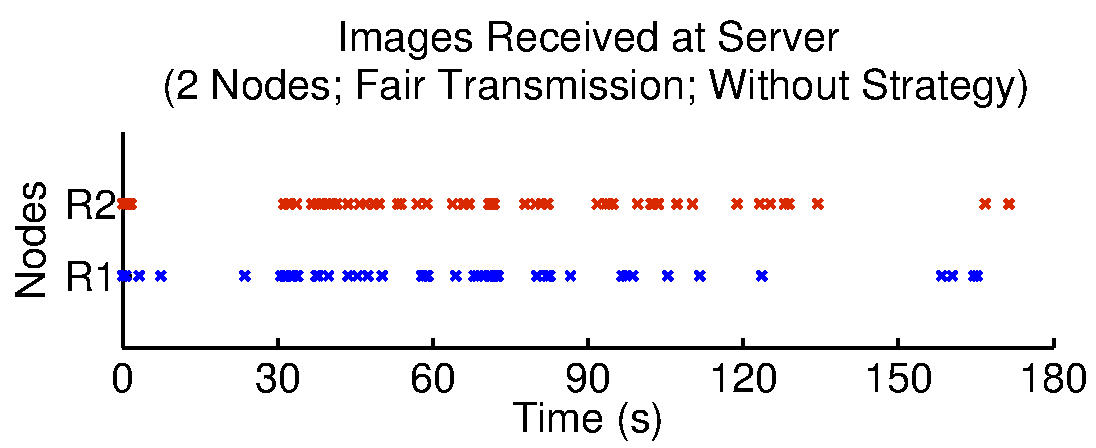
\includegraphics[width=\columnwidth]{Tex_Picts/MATLAB_Figs/LevelE/2Nodes/WITHOUT_Strategy/scatter_plot_of_transmission.pdf} 
%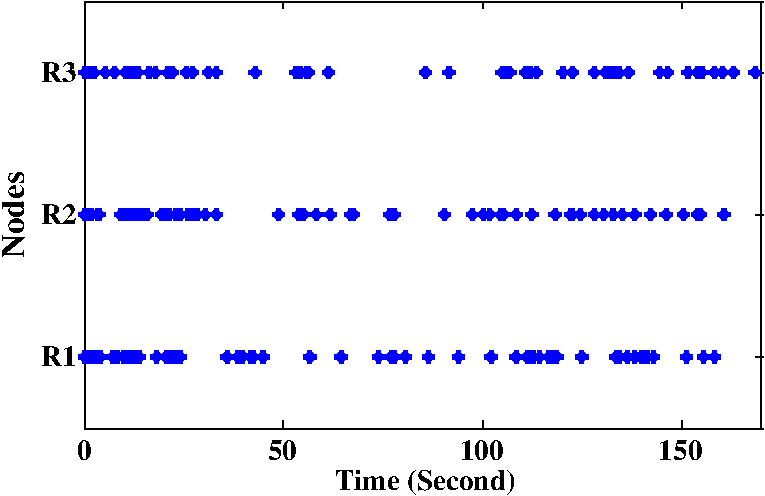
\includegraphics[width=0.8\columnwidth]{figure/ftime_nostrategy_4nodes_fair.pdf} 
%\label{fig:node_transmission_sequence_LevelE_2nodes_fair_noStrategy}
%	}
%\subfigure[With strategy]{
%%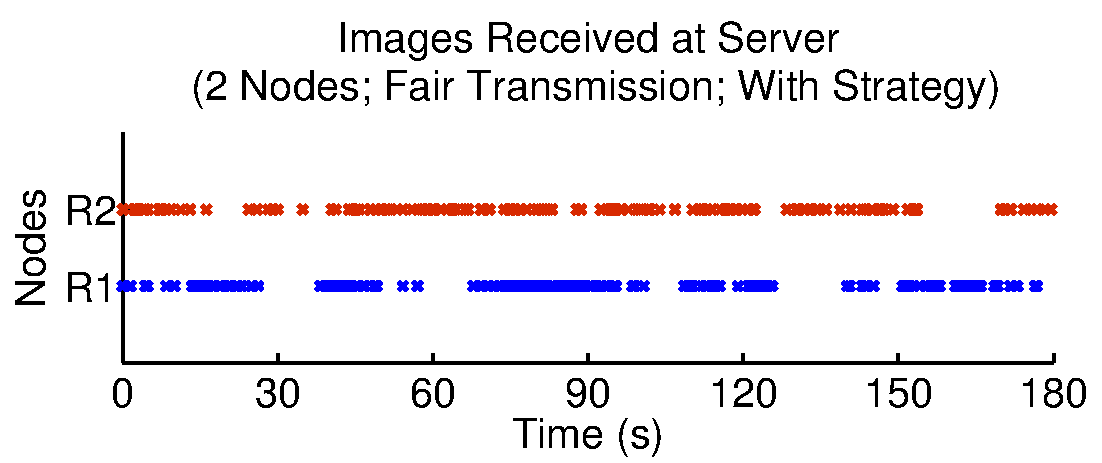
\includegraphics[width=\columnwidth]{Tex_Picts/MATLAB_Figs/LevelE/2Nodes/WITH_Strategy/scatter_lot_node_transmissions.pdf} 
%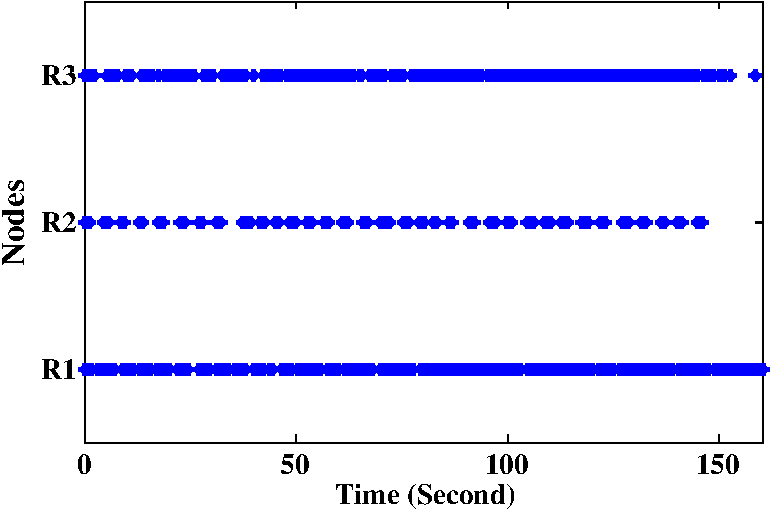
\includegraphics[width=0.8\columnwidth]{figure/ftime_withstrategy_4nodes_fair.pdf} 
%\label{fig:node_transmission_sequence_LevelE_2nodes_fair_withStrategy}
%	}
%\caption{Trace of images received at server (3 nodes; Fair Transmission)}
%\label{fig:trace_fair_levelE}
%%\vspace{-5mm}
%\end{figure}
%
%Traces of received images are demonstrated in Fig. \ref{fig:trace_fair_levelE}.
%Under significant WiFi interference, the RT-WMP alone is unable to deliver many
%images from the nodes to the server as shown in Fig.
%\ref{fig:node_transmission_sequence_LevelE_2nodes_fair_noStrategy}. 
%However, with the resource allocation strategy incorporated,  
%the periodic breaks in the entire duration of the transmission demonstrate the
%  improvement of fair bandwidth allocation among the three nodes in the trace
%  of images received at the server, as depicted in Fig.
%  \ref{fig:node_transmission_sequence_LevelE_2nodes_fair_withStrategy}.
%%Furthermore, the resource allocation strategy is actively attempting to
%%allocate the network between the three nodes as fairly as possible, 
%Moreover, the number of images correctly delivered to the server is shown in
%  Table \ref{tab:received_number_images}. 
%The values show that the strategy sharply increased the performance both in the
%three-node case and six-node case. 
%
%In principle, the RT-WMP is already fair in the sense that all the nodes have
%the same opportunity to transmit. It is granted by the fact that same-priority
%queued messages are selected according to their waiting time. 
%This means that, if all the nodes generate a message with the same priority at
%exactly the same moment, these messages will be selected one after the other in
%subsequent rounds.
%The reason for which in the first experiment shown in Fig.
%\ref{fig:node_transmission_sequence_LevelE_2nodes_fair_noStrategy} very few
%messages are delivered, is that images are split in several RT-WMP packets and
%all of them have to be received in order to recompose it.  
%If the traffic is saturated, the queues are likely full, and
%most of the messages are discarded at the moment of enqueueing.
%This means that, often, only part of an image is enqueued and it is
%impossible to recompose it.
%Then the messages can be retransmission a fixed number of time when the node
%sends a frame but does not receive an implicit acknowledgement within timeout.
%Therefore, the node receives less number of messages in a period of time than
%expected. 
%The use of the strategy alleviates this problem since it guarantees to one of
%the nodes a window in which that particular node has the right to transmit,
%thereby improving the global behavior as Fig. 
%  \ref{fig:node_transmission_sequence_LevelE_2nodes_fair_withStrategy}
%demonstrates.
%%
%%
%\begin{figure}[t]
%\centering
%\subfigure[No strategy]{
%%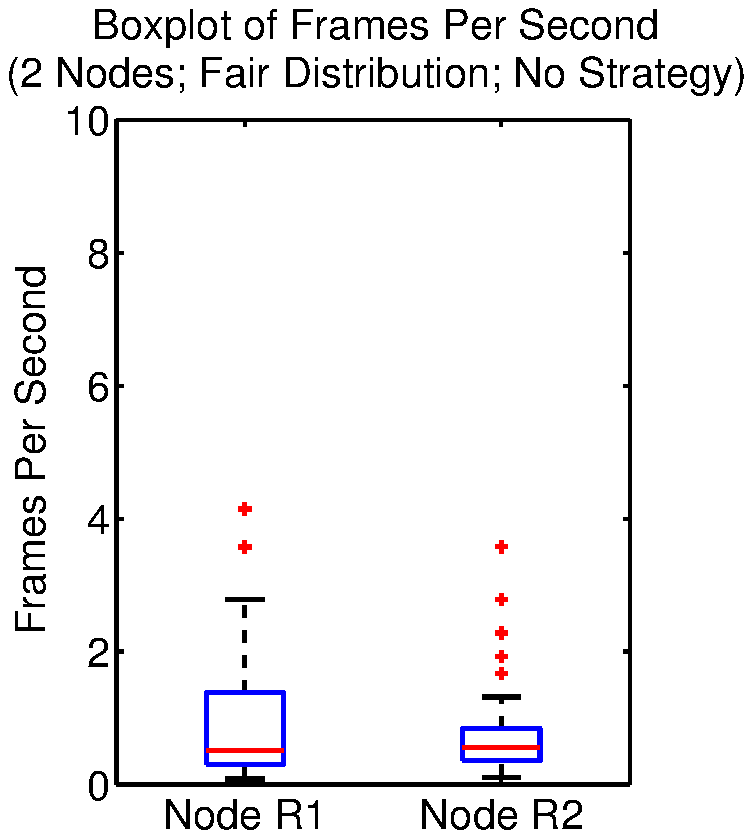
\includegraphics[width=0.45\columnwidth]{Tex_Picts/MATLAB_Figs/LevelE/2Nodes/WITHOUT_Strategy/boxplot_R1andR2_fps.pdf} 
%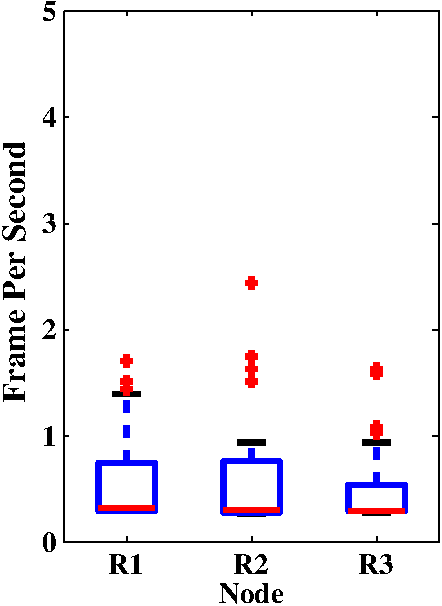
\includegraphics[height=0.62\columnwidth]{figure/fps_nostrategy_4nodes_fair.pdf} 
%\label{fig:boxplot_LevelE_3nodes_fair_noStrategy}
%				}
%\subfigure[With strategy]{
%%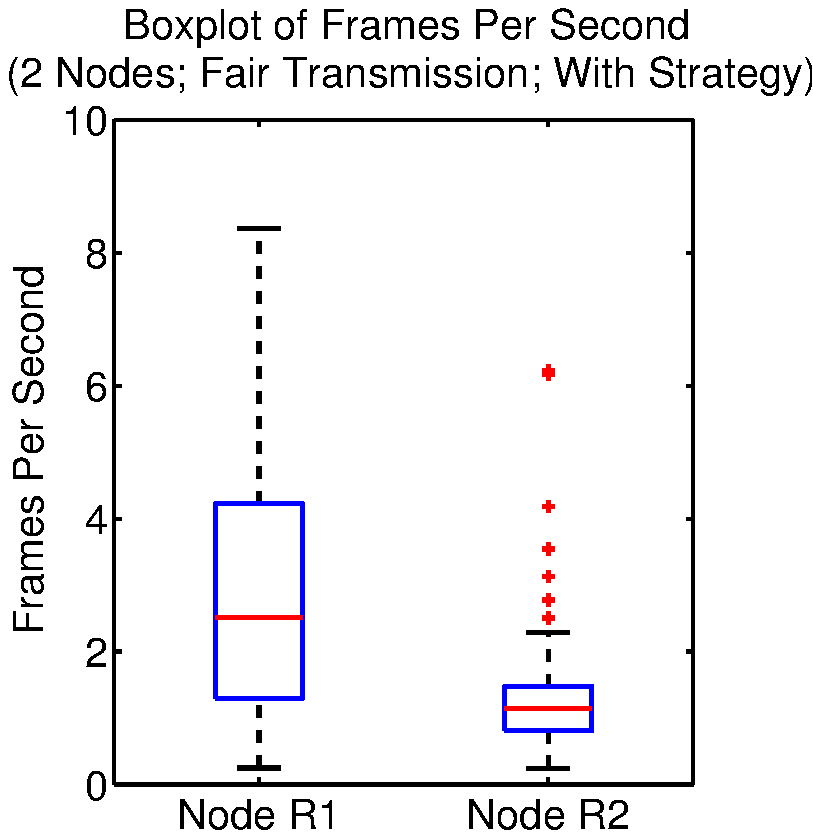
\includegraphics[width=0.45\columnwidth]{Tex_Picts/MATLAB_Figs/LevelE/2Nodes/WITH_Strategy/boxplot_R1andR2_fps.pdf} 
%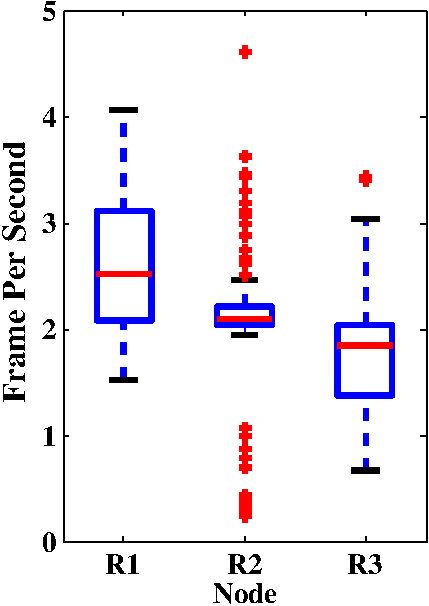
\includegraphics[height=0.62\columnwidth]{figure/fps_withstrategy_4nodes_fair.pdf} 
%\label{fig:boxplot_LevelE_3nodes_fair_withStrategy}
%				}
%\caption{Boxplots of FPS values (3 nodes; Fair Transmission)
%Red lines mark the median value. The edges of the blue box are the
%  25th and 75th percentiles, Black lines mark some extreme data points. This
%  representation applies for Fig. \ref{fig:fps_biased})
%}
%%\vspace{-3mm}
%\end{figure}
%
%Furthermore, a statistical comparison of Fig.
%  \ref{fig:boxplot_LevelE_3nodes_fair_noStrategy} and Fig.
%  \ref{fig:boxplot_LevelE_3nodes_fair_withStrategy} also indicates a
%  significant improvement in the performance of the network. 
%When no strategy is applied, the median FPS values for R1, R2 and R3 are 0.35,
%     0.31 and 0.30 respectively.
%However, with the resource allocation strategy applied, the median FPS values
%increased to 2.51, 2.11 and 1.91, respectively.
%In other words, the performance of R1, R2 and R3 increased by close to seven
%times, eight times and six times. 
%Hence, one can conclude the effectiveness of the resource allocation strategy
%under cases of significant WiFi interference.

%-------------------------------------------------------
% Figure
%-------------------------------------------------------
\begin{figure}[t]
\centering
\subfigure[No strategy]
{
%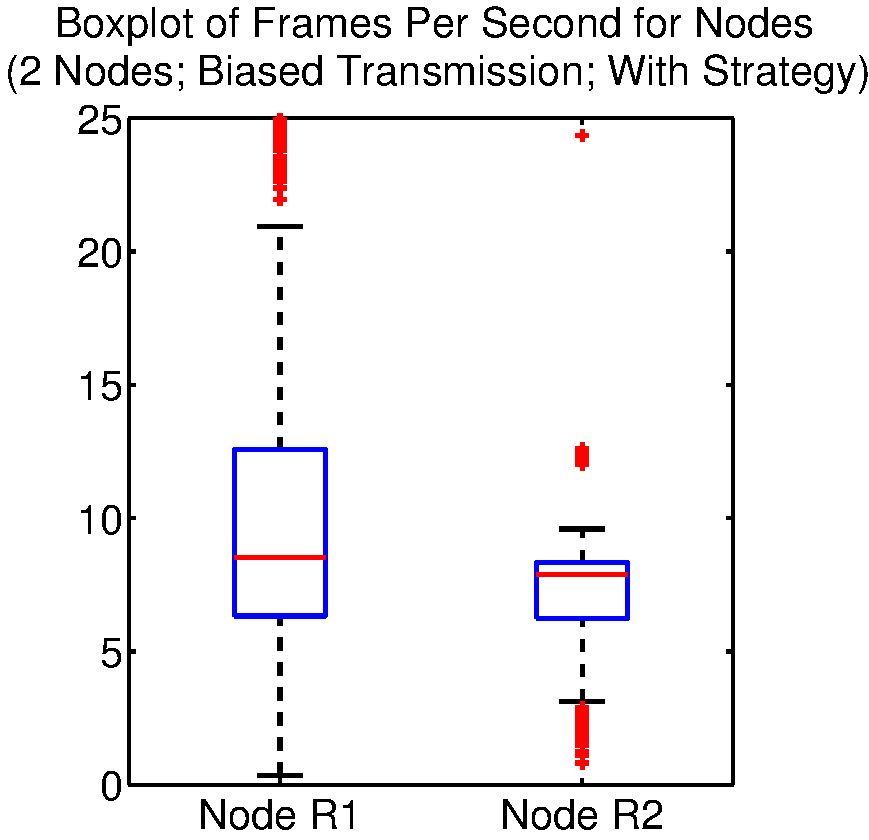
\includegraphics[width=0.45\columnwidth]{Tex_Picts/MATLAB_Figs/LevelA/Biased_Transmission/2Nodes/WITH_Strategy/boxplot_R1andR2_fps.pdf} 
%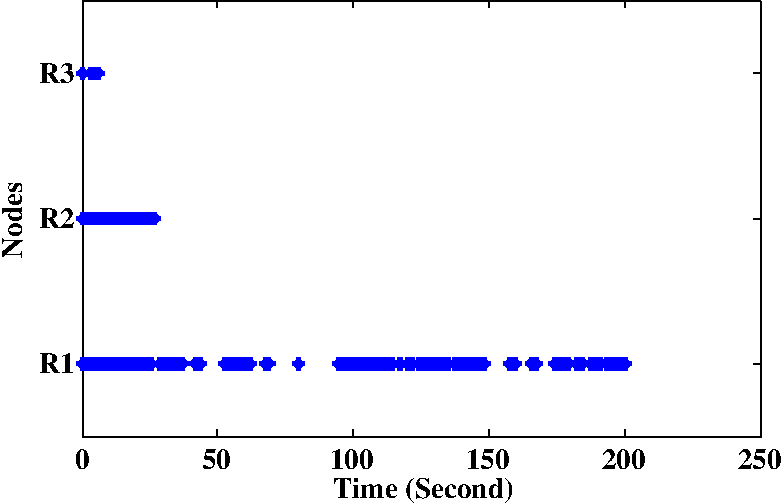
\includegraphics[width=0.80\columnwidth]{figure/ftime_nostrategy_4nodes_biased.pdf} 
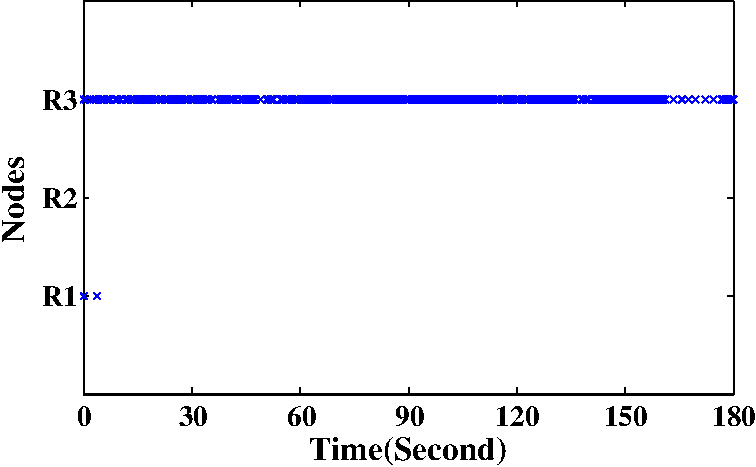
\includegraphics[width=0.80\columnwidth]{Tex_Picts/MATLAB_Figs/LevelA/Biased_Transmission/3Nodes/WITHOUT_Strategy/node_transmission_sequence.pdf} 
\label{fig:node_transmission_sequence_LevelA_2nodes_biased_noStrategy}
				}
\subfigure[With strategy]{
%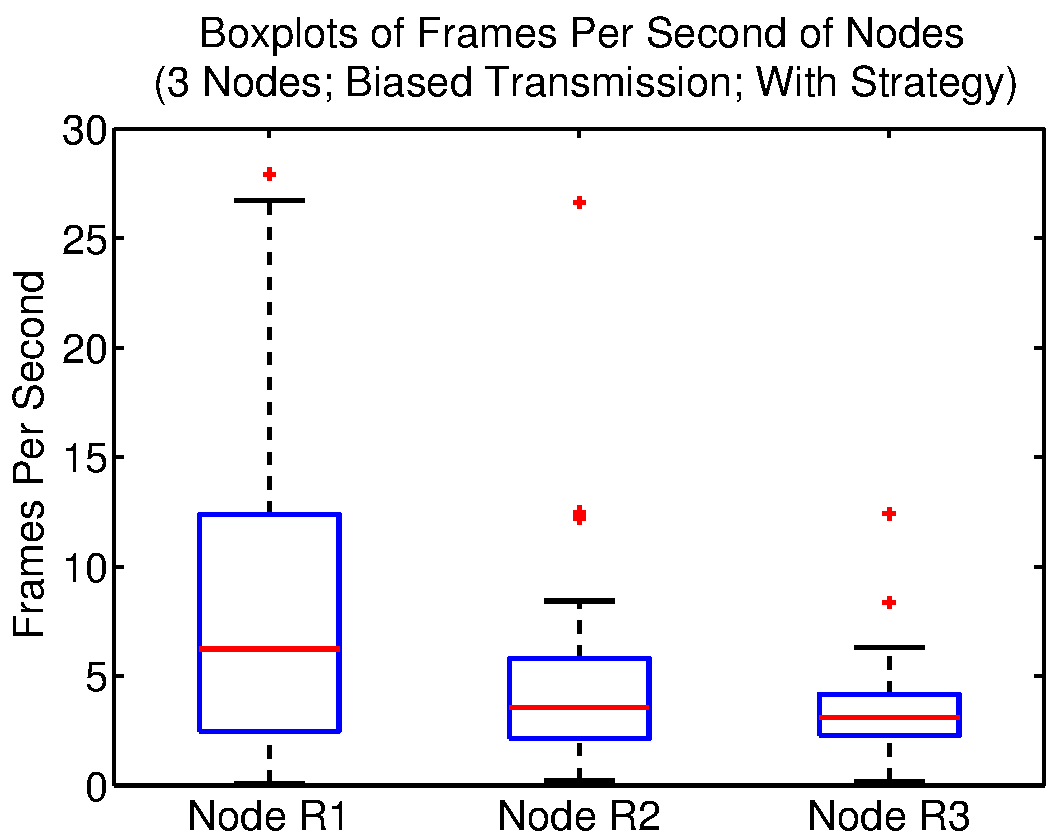
\includegraphics[width=0.45\columnwidth]{Tex_Picts/MATLAB_Figs/LevelA/Biased_Transmission/3Nodes/WITH_Strategy/boxplots_R1andR2andR3_fps.pdf} 
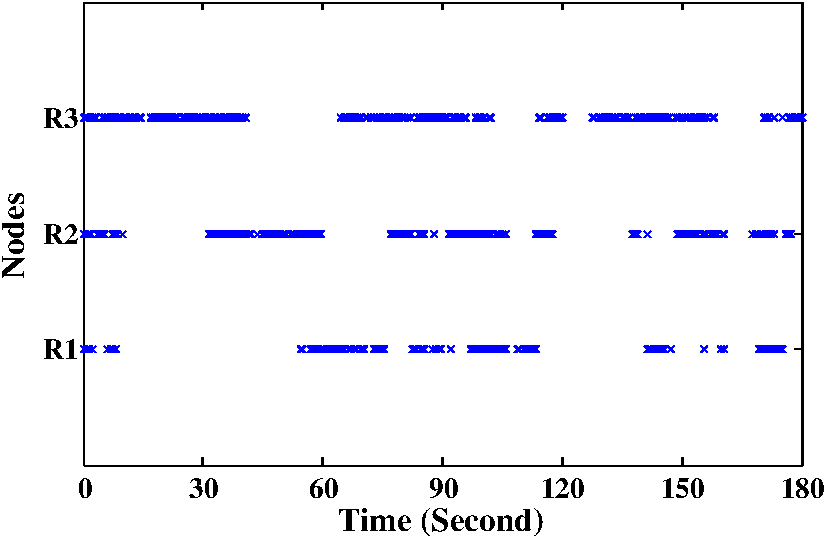
\includegraphics[width=0.80\columnwidth]{Tex_Picts/MATLAB_Figs/LevelA/Biased_Transmission/3Nodes/WITH_Strategy/node_transmission_sequence.pdf} 
%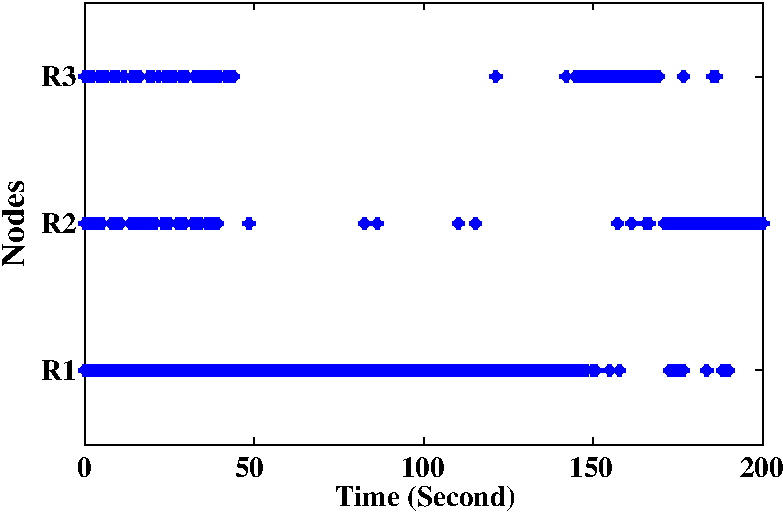
\includegraphics[width=0.80\columnwidth]{figure/ftime_withstrategy_4nodes_biased.pdf} 
\label{fig:node_transmission_sequence_LevelA_2nodes_biased_withStrategy}
				}
\caption{Trace of images received at server (3 nodes; Biased Transmission). }
\label{fig:trace_biased_3nodes}
%\vspace{-4mm}
\end{figure}
%-------------------------------------------------------

%-------------------------------------------------------
\begin{figure}[htpb]
\centering
\subfigure[No strategy]{
%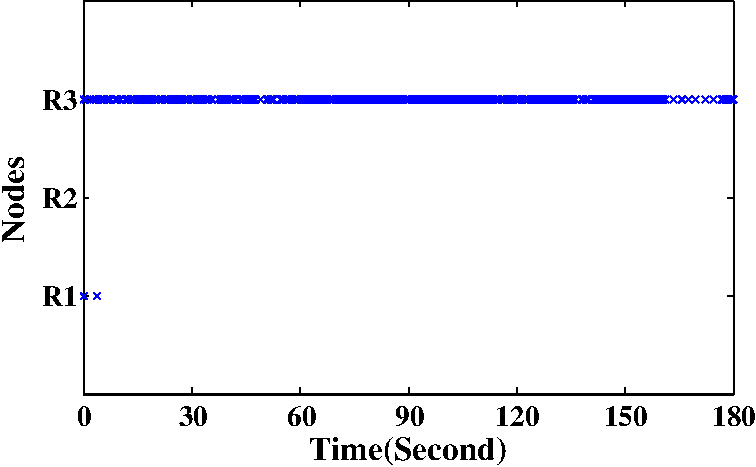
\includegraphics[width=0.80\columnwidth]{Tex_Picts/MATLAB_Figs/LevelA/Biased_Transmission/3Nodes/WITHOUT_Strategy/node_transmission_sequence.pdf} 
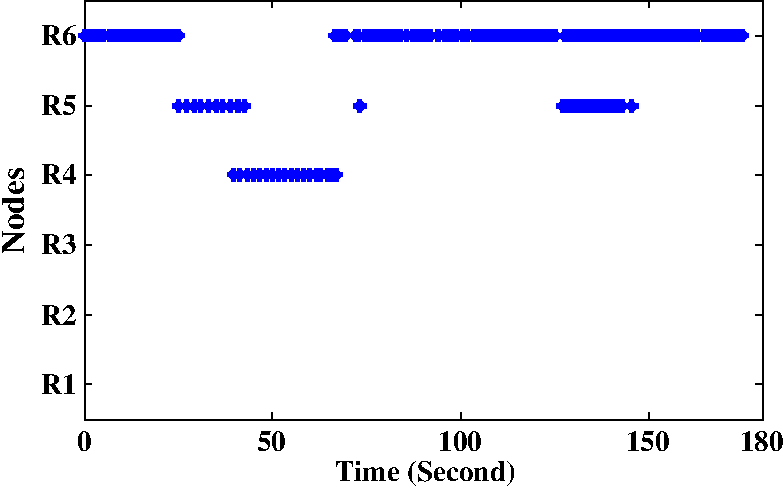
\includegraphics[width=0.80\columnwidth]{figure/ftime_nostrategy_7nodes_biased.pdf} 
\label{fig:node_transmission_sequence_6nodes_biased_noStrategy}
				}
  ~ %add desired spacing between images, e. g. ~, \quad, \qquad etc.
    %(or a blank line to force the subfigure onto a new line)
\subfigure[With strategy]{
%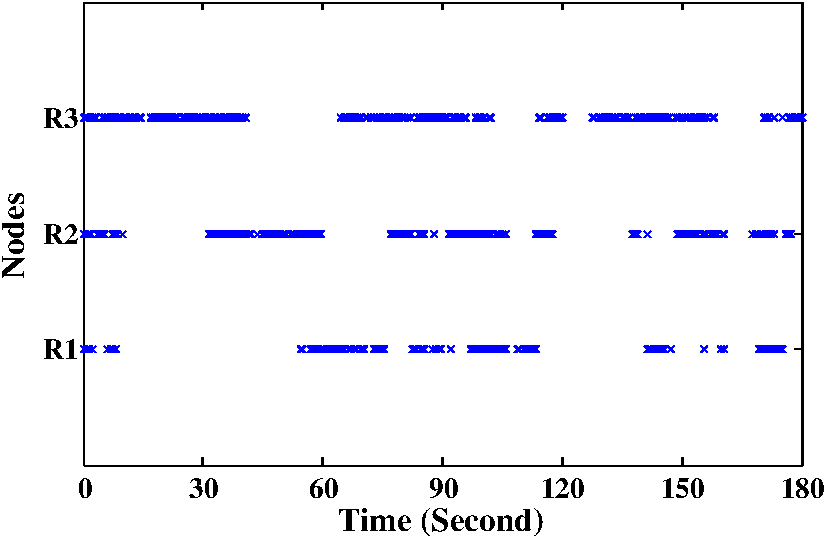
\includegraphics[width=0.80\columnwidth]{Tex_Picts/MATLAB_Figs/LevelA/Biased_Transmission/3Nodes/WITH_Strategy/node_transmission_sequence.pdf} 
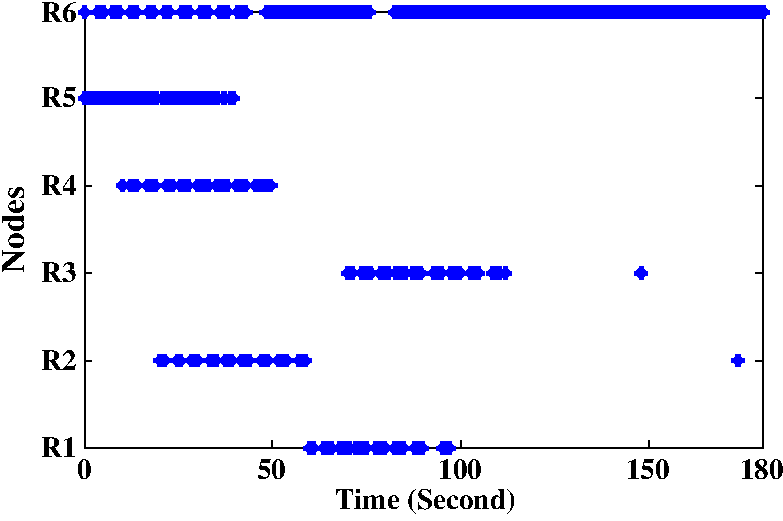
\includegraphics[width=0.80\columnwidth]{figure/ftime_7_S_B_favor.pdf} 
%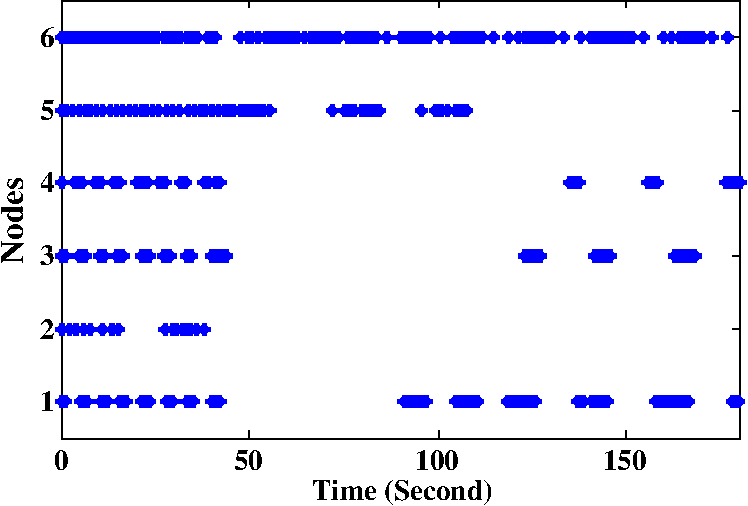
\includegraphics[width=0.80\columnwidth]{figure/ftime_withstrategy_7nodes_biased.pdf} 
\label{fig:node_transmission_sequence_6nodes_biased_withStrategy}
				}
\caption{Trace of images received at server (6 nodes; Biased Transmission)}
\label{fig:trace_biased_6nodes}
%\vspace{-3mm}
\end{figure}
%-------------------------------------------------------


%-------------------------------------------------------
% Table
%-------------------------------------------------------
\begin{table}[htpb]
\small
\caption{Received Number of Images at Server from Each Node}
\label{tab:nodes}
\centering
\begin{tabular}{ccccc}
%\begin{tabular}{p{0..05\textwidth}p{0.1\textwidth}p{0.1\textwidth}p{0.1\textwidth}p{0.1\textwidth}p{0.1\textwidth}p{0.1\textwidth}p{0.05\textwidth}p{0.1\textwidth}}
\toprule
%\multirow{3}{*}{\text{Nodes}} & \multicolumn{4}{c}{\text{Biased Transmission}} \\
%\cmidrule(r){2-5}
 \multirow{3}{*}{\text{Nodes}}& \multicolumn{2}{c}{\text{3 Nodes}} & \multicolumn{2}{c}{\text{6 Nodes}}  \\
\cmidrule(r){2-5}
 &  No  & With  & No  & With  \\
 &   Strategy & Strategy  &  Strategy &  Strategy \\
%  No \newline{Strategy} & With \newline{Strategy} & No \newline{Strategy} & With \newline{Strategy} \\
\midrule
R1  &8 &276 &0   &62  \\ %167 \\ 
R2  &0 &232 &0   &81  \\ %242 \\ 
R3  &815&521&0   &151 \\ % 134 \\ 
R4  &-  &-  &18  &74  \\ %125 \\ 
R5  &-  &-  &29  &69  \\ %210 \\ 
R6  &-  &-  &190 &756 \\ % 289 \\ 
\bottomrule
\label{tab:received_number_images}
\end{tabular}
\end{table}

%\subsubsection{Biased Transmissions}
In the \textit{Biased Transmission}, 
one node was set as the favored node and has the highest priority throughout
the whole trace of transmission  when no
strategy is applied; 
on the other hand, the proposed strategy can dynamically change the priority of
the favored node to improve the performance of the network. 

Traces of received images are demonstrated in Fig.
\ref{fig:trace_biased_3nodes} and Fig. \ref{fig:trace_biased_6nodes}.
For a three-node setup, it can be observed that configuring R3 to have the
highest priority throughout the transmission session almost prevents R2 and R1
from transmitting when no strategy applied as shown in Fig.
\ref{fig:node_transmission_sequence_LevelA_2nodes_biased_noStrategy}.
For a six-node setup, a similar outcome is shown in Fig.
\ref{fig:node_transmission_sequence_6nodes_biased_noStrategy}, when R6
has its priority set to be the highest in the network. 
It is clear to conclude that without the resource allocation strategy, a biased
transmission will only allow the favored node to transmit and effectively halt
the transmission from other nodes.
On the other hand, when the resource allocation strategy is applied, the
favored node is still allowed to transmit for the bulk of the transmission
period, while other non-favored nodes could still transmit periodically,
  at a shorter frequency (see Fig.
\ref{fig:node_transmission_sequence_LevelA_2nodes_biased_withStrategy}
and Fig. \ref{fig:node_transmission_sequence_6nodes_biased_withStrategy}).
Thus, the strategy clearly achieves its goal of allowing other non-favored
nodes to transmit periodically.

Moreover, the number of images correctly delivered to the server is shown in
Table \ref{tab:received_number_images} for \textit{Biased Transmission} as
well. 
%The values demonstrate that the strategy increased the performance about 5 times in 
%the three-node case, about 10 times for non-favored nodes and about 1.5 times for 
%the favored node R6 in the six-node case. 
The values demonstrate that the strategy enables the favored node transmits
most images, and other nodes transmit some images regarding their priorities
both in the three-node case and in the six-node case. 


\begin{figure}[t]
\centering
\subfigure[No strategy]
{
%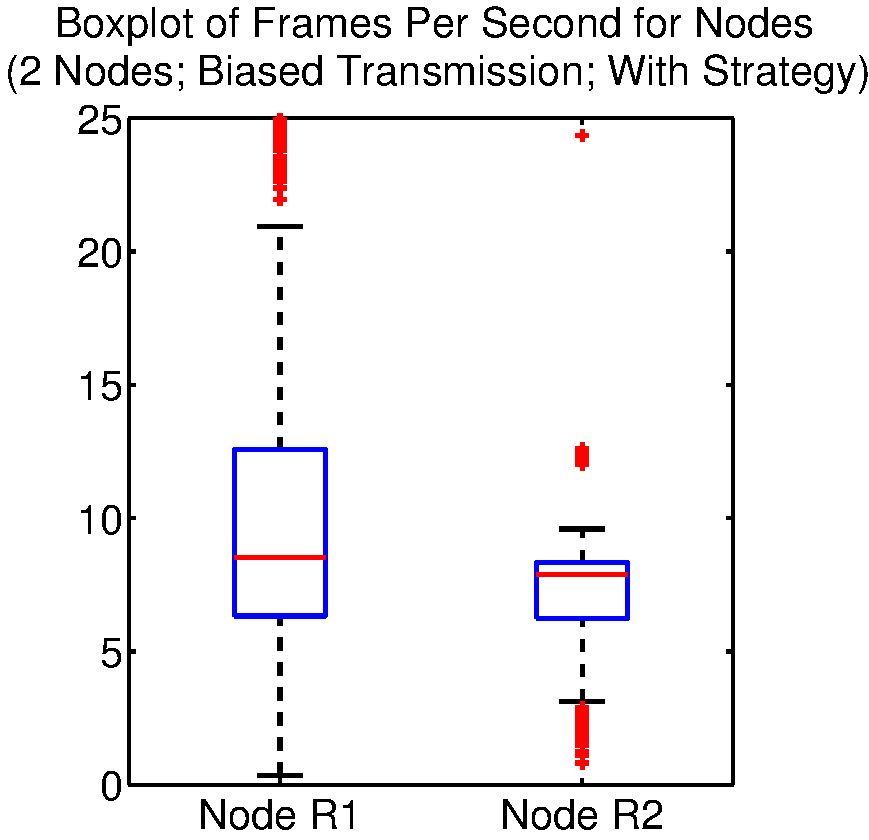
\includegraphics[width=0.45\columnwidth]{Tex_Picts/MATLAB_Figs/LevelA/Biased_Transmission/2Nodes/WITH_Strategy/boxplot_R1andR2_fps.pdf} 
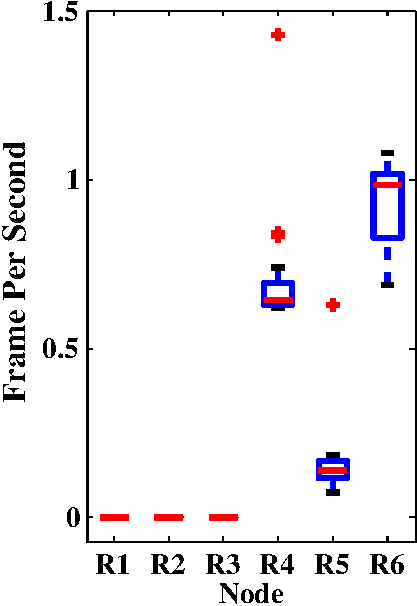
\includegraphics[height=0.62\columnwidth]{figure/fps_nostrategy_7nodes_biased.pdf} 
\label{fig:boxplot_6nodes_biased_noStrategy}
%\label{fig:boxplot_LevelA_2nodes_biased_noStrategy}
				}
  %
  ~ %add desired spacing between images, e. g. ~, \quad, \qquad etc.
    %(or a blank line to force the subfigure onto a new line)
\subfigure[With strategy]{
%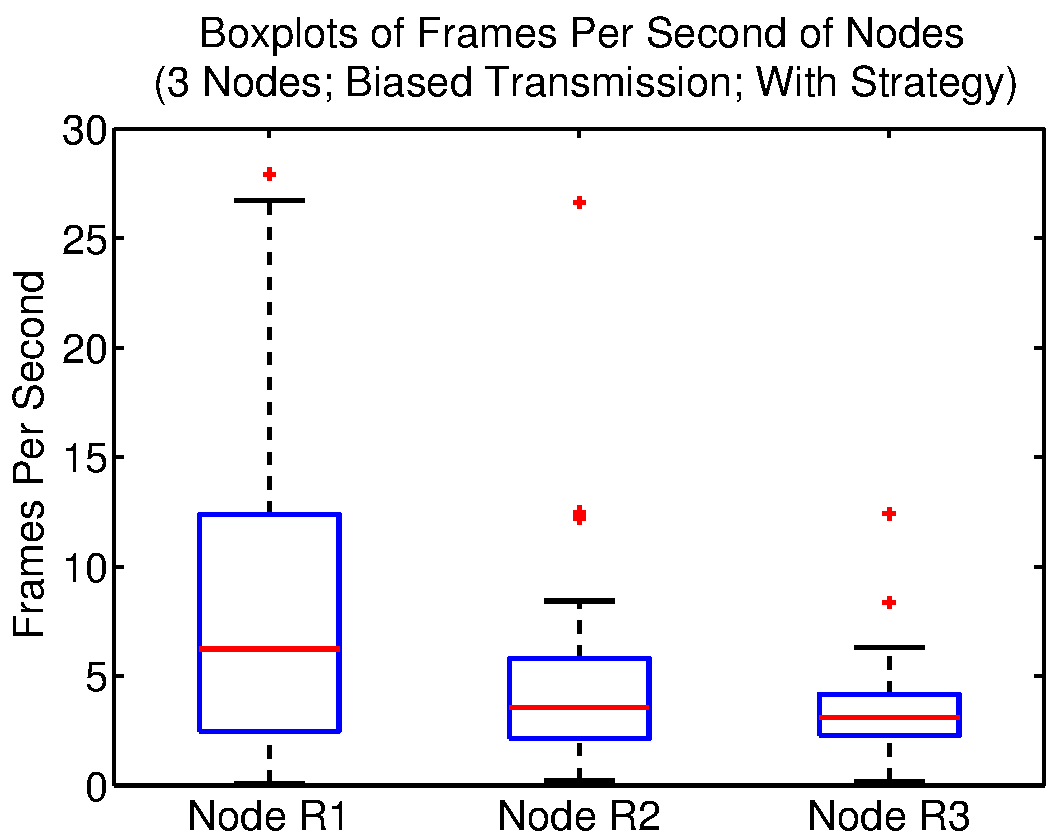
\includegraphics[width=0.45\columnwidth]{Tex_Picts/MATLAB_Figs/LevelA/Biased_Transmission/3Nodes/WITH_Strategy/boxplots_R1andR2andR3_fps.pdf} 
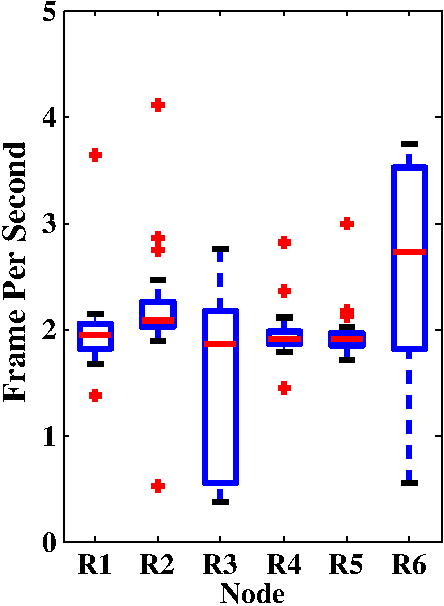
\includegraphics[height=0.62\columnwidth]{figure/fps_7_S_B.pdf} 
%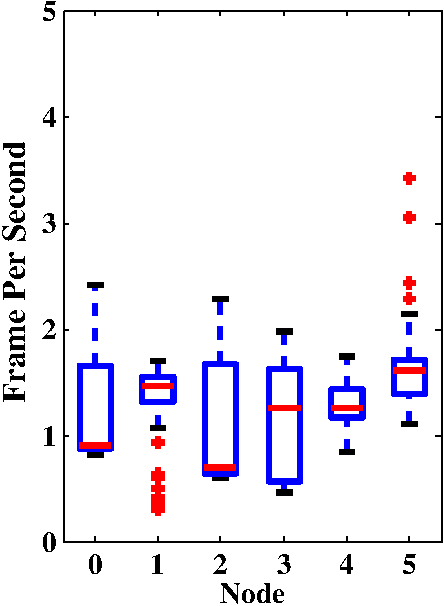
\includegraphics[height=0.65\columnwidth]{figure/fps_withstrategy_7nodes_biased.pdf} 
\label{fig:boxplot_6nodes_biased_withStrategy}
%\label{fig:boxplot_LevelA_3nodes_biased_withStrategy}
				}
\caption{Boxplots of FPS values (6 nodes).
Red lines mark the median value. The edges of the blue box are the
  25th and 75th percentiles, Black lines mark some extreme data points.}
\label{fig:fps_biased}
%\vspace{-3mm}
\end{figure}

%For the three-node setup, the median FPS values are 6.23, 3.57 and 3.12,
%respectively as shown in  Fig. \ref{fig:boxplot_3nodes_biased_noStrategy}. 
%%This indicates that the performance of R3 is extremely similar to that of R2,
%%     even though R1 has much fewer opportunities to transmit. 
%%Note that the larger range of FPS values seen in R1 is expected.
%%Because it is unable to transmit for significantly long periods of time, the
%%proxy reports a decreased FPS value from R1. 
%%At the same time, the data
%%packets produced at R1 would be queued up. Once R1 is given the priority to
%%transmit, these queued up data packets are transmitted to the proxy as
%%quickly as possible, at a rate higher than the camera frame rate. Thus, with
%%the sudden rush of images being received at the proxy, it reports larger FPS
%%values at those instants. 
%%
%In particular, considering that the number of images received from R1 at the
%server is the lowest, the median FPS value is found to be higher than that of
%R2 and R3, surprisingly. 
%This is due to the long time periods when R1 was unable to transmit, at the
%intervals $t\in[8,54]$ and $t \in [113, 141]$.
%These long time periods result in an extremely long queue of packets in the
%node. 
%During the extremely short time periods when R1 is allowed to transmit, the
%rapid arrival of packets at the server causes the FPS values to be extremely
%high.
%As this transmission period is extremely short, there is insufficient time to
%clear the transmission queue at R1 and the data flow between R1 and the server
%could not be reduced back to the normal rate.
%This accounts for the higher median FPS value in R1.
%
%On the other hand, the median FPS values of R2 and R3 are extremely similar. 
%In fact, as shown in Fig. 
%\ref{fig:node_transmission_sequence_LevelA_2nodes_biased_withStrategy}, while
%R3, which is the favored node, clearly takes up the bulk of the time, R2
%appeared to transmit for an amount of time that is less, but close to that of
%R3. 
%Indeed, one can observe significant ``overlap'' in transmissions between
%R2 and R3. 
%This is due to how the RT-WMP handles different data flows when the network is
%not saturated. As expected, the RT-WMP allows the node with the highest
%priority data flow in a given instant (say, R3) to transmit. 
%However, if the highest priority data flow does not saturate the bandwidth,
%  such that there is sufficient amount of bandwidth available to accommodate a
%  second data stream of lower priority, then the RT-WMP would allow this data
%  stream to be transmitted simultaneously. 
%Thus, this explains why there is a significant amount of simultaneous
%transmissions between R2 and R3, resulting in similar median FPS values, and
%hence, similar performances for these three nodes.

In addition, a statistical comparison of Fig.
\ref{fig:boxplot_6nodes_biased_noStrategy} and Fig.
\ref{fig:boxplot_6nodes_biased_withStrategy} also indicates a significant
improvement in the performance of the number of received images. 
When no strategy is applied, the median FPS values for R1 to R6 are 0,
 0, 0, 0.64, 0.14 and 0.98, respectively.  
However, with the resource allocation strategy applied, the median FPS values
are increased to 1.95, 2.01, 1.86, 1.90, 1.91 and 2.72, respectively.
Therefore, the favored node has higher median FPS and transmitted the images
more stable than other nodes.
Meanwhile, other nodes have transmitted some images 
with a relatively similar rate.

%The reasons of effectiveness of the resource allocation strategy
%under cases of significant WiFi interference are as follows:
In particular, 
R6 is mostly the favored node during the test because it took up the bulk of
the time to transmit images as shown in Fig.
\ref{fig:node_transmission_sequence_6nodes_biased_withStrategy}.
%However, it transmitted more number of images compared to the case when it set
%up to be the highest priority with no strategy applied as shown in Fig. 
\ref{fig:boxplot_6nodes_biased_withStrategy}.
The reason is as follows:
\begin{itemize}
\item 
RT-WMP handles several data flow from other nodes from time to time beside the
favored node when the network is not saturated;
 once the traffic is saturated, the queues are likely full or almost full, and
 most of the messages are discarded at the moment of queueing; 
\item
 Images in the data flow are split in several RT-WMP packets and all of them
 have to be received in order to recompose it;  
the discarded packets in the queue results in only part of an image that is
enqueued. As such, it is impossible to recompose the full image, hence, the
image cannot be received by the receiver.
\end{itemize}

\section{Conclusion}
\label{sec:conclusion}

This paper has formulated an optimization problem of resource allocation
including a non-convex cost function and time constraint.
We have presented an incremental auction-based resource allocation strategy
that runs in conjunction with the RT-WMP.
The proposed approach adopts a leaderless consensus procedure to share the bids
among the networked robots. 
Each robot in the system locally bids for a quantity of transmission time slots
in a distributed manner. 
By default, it attempts to allocate the network resource fairly among the nodes
in a cloud robotic system, but if the user chooses to scrutinize a particular
node instead, the strategy can adapt to that request.
We have proved the optimal of the proposed strategy theoretically. 
It was also tested on an ad-hoc network situated in typical indoor environments
to gauge its performance, which was compared to the cases whereby no strategy
was used (i.e. an uncontrolled network).
A different number of nodes were used to gauge how well the strategy worked
under different loads. The experimental results showed that the nodes were
still able to transmit images to the server at a reasonable FPS value even with
significant WiFi interference with assistance from the resource
allocation strategy.
The resource allocation strategy has also met its two-fold
aim of allocating the network resource to all nodes as fairly as possible, as
well as letting other non-favored nodes transmit periodically, at a lower
frequency. 

Future development of this contribution includes developing optimization 
algorithms that are able to tune the strategy according to the additional 
tasks and implementations.

%Future development on this contribution includes developing optimisation
%algorithms that are able to tune the variables in the strategy according to the
%network topology, the number of nodes in the network and the amount of
%interference on the system. This will then increase the robustness of this
%resource allocation strategy to make it suitable for all environments and
%applications.

%\begin{acknowledgements}
%If you'd like to thank anyone, place your comments here
%and remove the percent signs.
%\end{acknowledgements}

% BibTeX users please use one of
%\bibliographystyle{spbasic}      % basic style, author-year citations
%\bibliographystyle{spmpsci}      % mathematics and physical sciences
\bibliographystyle{IEEEtran}      % mathematics and physical sciences
%\bibliographystyle{spphys}       % APS-like style for physics
\bibliography{lujia_main}   % name your BibTeX data base

% Non-BibTeX users please use
%\begin{thebibliography}{}
%%
%% and use \bibitem to create references. Consult the Instructions
%% for authors for reference list style.
%%
%\bibitem{RefJ}
%% Format for Journal Reference
%Author, Article title, Journal, Volume, page numbers (year)
%% Format for books
%\bibitem{RefB}
%Author, Book title, page numbers. Publisher, place (year)
%% etc
%\end{thebibliography}
%
\end{document}
% end of file template.tex

